\subsection{不可分解模与原始模}

设 A 是一个环。回忆下面的定义（VII, §4, No.~8, 第 23 页，定义 3）。

定义 2. —— 若 A-模 M 不是一族异于 0 与 M 的子模的直和，则称 A-模 M 为不可分解模。

由 II, §1, No.~8, 第 209 页命题 12 的推论，下列性质等价：

\begin{enumerate}
\def\labelenumi{\alph{enumi})}
\item
  A-模 M 不可分解。
\item
  A-模 M 非零，且 M 的每个作为直因子的子模都等于 0 或 M。
\item
  A-模 M 非零，且环 \(\operatorname{End}_{\mathrm{A}}(\mathrm{M})\) 不含异于 0 和 \(1_{M}\) 的幂等元。
\end{enumerate}

特别地，由于 A-模 \(A_{s}\) 的自同态环同构于 A 的反环，我们可见 A-模 \(A_{s}\) 不可分解当且仅当环 A 非零且其仅有的幂等元是 0 和 1。

例. —— 设环 A 是主理想整环。不可分解的有限生成 A-模是同构于 A 或 \(A/p^{n}A\) 的那些 A-模，其中 p 是 A 的不可约元，n 为整数 \textgreater0（VII, §4, No.~8, 第 24 页，命题 8）。

命题 3. —— 诺特的或阿廷的 A-模 M 是不可分解子模的有限族的直和。

先证明 M 的每个非零子模 P 都有一个不可分解的直因子。若不然，则 P 的每个直因子子模都是可分解的；于是用归纳法，可对每个 \(n \in N\) 构造 P 的非零子模 \(N_{n}^{\prime}\) 与 \(N_{n}^{\prime\prime}\)，使得 \(P = N_{0}^{\prime} \oplus N_{0}^{\prime\prime}\) 且 \(N_{n-1}^{\prime} = N_{n}^{\prime} \oplus N_{n}^{\prime\prime}\)（\(n \geqslant 1\)）。但这样一来，子模序列 \(N_{0}^{\prime\prime} + \cdots + N_{n}^{\prime\prime}\) 将严格递增，而子模序列 \(N_{n}^{\prime}\) 将严格递减。于是模 M 既非诺特的亦非阿廷的，与假设矛盾。

现在设 M 不是不可分解子模的有限族的直和。用归纳法，我们构造 M 的不可分解子模 \(P_{n}^{\prime\prime}\) 与 M 的非零子模 \(P_{n}^{\prime}\)（对每个 \(n \in N\)），使得 \(M = P_{0}^{\prime} \oplus P_{0}^{\prime\prime}\) 且 \(P_{n-1}^{\prime} = P_{n}^{\prime} \oplus P_{n}^{\prime\prime}\)（\(n \geqslant 1\)）。事实上，M 非零，把证明的第一部分应用于 P = M，即得到 \(P_{0}^{\prime}\) 与 \(P_{0}^{\prime\prime}\)。由于模 \(P_{k}^{\prime}\) 与 \(P_{k}^{\prime\prime}\) 对 k \textless{} n 已有定义，由证明的第一部分，存在子模 \(P_{n}^{\prime}\) 与 \(P_{n}^{\prime\prime}\)，使得 \(P_{n-1}^{\prime} = P_{n}^{\prime} \oplus P_{n}^{\prime\prime}\)，其中 \(P_{n}^{\prime\prime}\) 不可分解。因为 M 不是不可分解模的有限族的直和，关系式 \(M = P_{n}^{\prime} \oplus P_{0}^{\prime\prime} \oplus \cdots \oplus P_{n}^{\prime\prime}\) 便蕴含 \(P_{n}^{\prime} \neq 0\)。

子模序列 \(P_{0}^{\prime\prime} \oplus \cdots \oplus P_{n}^{\prime\prime}\) 严格递增，而子模序列 \(P_{n}^{\prime}\) 严格递减。这与 M 是诺特的或阿廷的这一假设相矛盾。

把模分解为不可分解子模的直和时的唯一性问题，将在下一小节中研究。

定义 3. —— 若一个模的自同态环是局部环，则称该模为原始模 \(^{(1)}\)。

按定义，局部环不化为 0；因此，原始模非零。此外，A-模 \(A_{s}\) 是原始模当且仅当环 A 是局部环。

命题 4. —— a) 原始模是不可分解模。

\begin{enumerate}
\def\labelenumi{\alph{enumi})}
\setcounter{enumi}{1}
\tightlist
\item
  有限长度的不可分解模是原始模。
\end{enumerate}

设 M 是一个 A-模。设 M 是原始模；设 e 是局部环 \(\operatorname{End}_{\mathrm{A}}(\mathrm{M})\) 中的一个幂等元。由于 \(e^{2}=e\)，或者 e 可逆从而 e=1，或者 1-e 可逆从而 e=0。这就证明 M 不可分解（VIII，第 30 页）。

现在设 M 不可分解且长度有限。由 VIII，第 27 页命题 2, c)，M 的每个自同态都可逆或幂零；于是环 \(\operatorname{End}_{\mathrm{A}}(\mathrm{M})\) 是局部环（VIII，第 26 页，例 2）。

Z-模 Z 不可分解、是诺特的，但不是阿廷的。它的自同态环同构于 Z，因而不是局部环。于是 Z 不是原始 Z-模。

*设 \(p\) 是素数。\(\mathbf{Z}\) -模 \(\mathbf{Q}_p / \mathbf{Z}_p\) 的自同态环同构于局部环 \(\mathbf{Z}_p\)（参见 VII, §4, 第 65 页，习题 13）；因此它是原始 \(\mathbf{Z}\) -模。

一个内射模不可分解当且仅当它是原始模（X, §1, n° 9, 第 21 页，命题 14）。*

\subsection{半原始模}

定义 4. —— 若一个模是原始子模的一个族的直和，则称它为半原始模。

*例. —— 1) 每个单模都是原始模（VIII，第 45 页）；因此每个半单模都是半原始模（VIII，第 55 页，定义 1）。

\begin{enumerate}
\def\labelenumi{\arabic{enumi})}
\setcounter{enumi}{1}
\tightlist
\item
  若 A 是左诺特环，则每个内射 A-模都是半原始的（X, §1, n° 9, 第 21 页，命题 14 及 X, §1, n° 10, 第 22 页，定理 3, b)）。*
\end{enumerate}

定理 1（阿祖马亚）. —— 设 A 是环，L 是原始 A-模，M 是半原始 A-模。存在唯一的基数，记作 {[}M : L{]}，它具有下列性质：

对 M 作为原始模的直和的每个分解 \(M = \bigoplus_{i \in I} M_i\)，指标 \(i \in I\) 中使 \(M_i\) 同构于 L 的那些指标组成的集合具有基数 {[}M : L{]}。

证明基于下面四个引理。

引理 1. —— 设 M 是一个 A-模，M' 是 M 的一个原始子模，M'\,' 是 M 中与 M' 互补的一个子模。设 u 是 M 的一个自同态。则 u 或 \(1_{M} - u\) 诱导出从 M' 到 M 中与 M'\,' 互补的一个子模的同构。

设 \(p\) 是 M 到 \(M'\) 上的、核为 \(M''\) 的投影，并设 \(v\) 是 \(p \circ u\) 在 \(M'\) 上的限制。先设 \(v\) 是 \(M'\) 的自同构。由于 \(v\) 是单射，\(u\) 在 \(M'\) 上的限制是单射，且我们有 \(u(M') \cap M'' = 0\)。由于 \(v\) 是满射，我们有 \(u(M') \oplus M'' = M\)。因此，\(u\) 诱导出从 \(M'\) 到 M 中与 \(M''\) 互补的一个子模的同构。现在设 \(v\) 不是 \(M'\) 的自同构。则 \(1_{M'} - v\) 是 \(M'\) 的自同构，因为 \(M'\) 是原始模。而 \(1_{M'} - v\) 是 \(p \circ (1_M - u)\) 在 \(M'\) 上的限制。前面的论证表明，\(1_M - u\) 诱导出从 \(M'\) 到 M 中与 \(M''\) 互补的一个子模的同构。

引理 2. —— 设 M 是一个 A-模，它是原始子模的族 \((\mathrm{M}_{i})_{i\in\mathrm{I}}\) 的直和，并设 u 是 M 的一个自同态。对 I 的每个子集 J，令 \(v=1_{M}-u\)，\(M_{J}=\bigoplus_{i\in J}M_{i}\)。则下列两个性质之一成立：

\begin{enumerate}
\def\labelenumi{\alph{enumi})}
\item
  存在一个指标 \(i \in I\)，使 u 诱导出从 \(M_{i}\) 到 M 的一个直因子子模的同构。
\item
  凡 \(J\) 是 \(I\) 的有限子集，\(v\) 都诱导出从 \(M_J\) 到与 \(M_{I-J}\) 互补的一个子模的同构。
\end{enumerate}

若性质 b) 成立，则 v 是单射。

设性质 a) 不成立，我们对 J 的基数用归纳法来确立性质 b)。若 \(J = \varnothing\)，则没有什么要证明的。于是设 J 非空，取 J 的一个元素 i，并令 \(J' = J - \{i\}\)。由归纳假设，v 诱导出从 \(M_{J'}\) 到 M 中与 \(M_{I-J'} = M_{I-J} \oplus M_i\) 互补的一个子模的同构；因此，子模 \(M'' = v(M_{J'}) \oplus M_{I-J}\) 与 \(M_i\) 互补。由引理 1 以及关于 u 的假设，自同态 v 诱导出从 \(M_i\) 到 M 中与 \(M''\) 互补的一个子模的同构；从而 v 诱导出从 \(M_J = M_i \oplus M_{J'}\) 到与 \(M_{I-J}\) 互补的一个子模的同构。

最后的断言来自如下事实：M 是诸子模 \(M_{J}\) 的并，其中 J 取遍 I 的有限子集。

引理 3. —— 设 M 是一个 A-模，它是原始子模的族 \((\mathrm{M}_{i})_{i\in\mathrm{I}}\) 的直和，并设 p 是 M 的一个非零投影算子。存在指标 \(i\in I\)，使 p 诱导出从 \(M_{i}\) 到 \(p(\mathrm{M})\) 的一个直因子子模的同构。

由于 p 非零，\(1_{M} - p\) 不是单射。由引理 2，存在指标 \(i \in I\)，使 p 诱导出从 \(M_{i}\) 到 M 的一个直因子子模的同构。M 的每个以 \(p(\mathrm{M}_{i})\) 为像的投影算子经限制都定义出 \(p(\mathrm{M})\) 的一个以 \(p(\mathrm{M}_{i})\) 为像的投影算子，故 \(p(\mathrm{M}_{i})\) 是 \(p(\mathrm{M})\) 的直因子子模。

引理 4. —— 设 M 是一个 A-模，它是原始子模的族 \((\mathrm{M}_{i})_{i\in\mathrm{I}}\) 的直和，设 L 是一个原始 A-模，并设 N 是 M 的一个直因子子模。设 N 是同构于 L 的子模的族 \((\mathrm{N}_{j})_{j\in\mathrm{J}}\) 的直和，并用 \(I_{L}\) 表示指标 \(i\in I\) 中使 \(M_{i}\) 同构于 L 的那些指标的集合。则有

\[
\operatorname{Card} (\mathrm{J}) \leqslant \operatorname{Card} \left(\mathrm{I} _ {\mathrm{L}}\right).\tag{1}
\]

设 \(N_0\) 是 M 中与 N 互补的一个子模。模 M 是 \(N_0\) 与族 \((N_j)_{j \in J}\) 的直和。对每个 \(j \in J\)，用 \(p_j\) 表示与这一分解相伴的、以 \(N_j\) 为像的 M 的投影算子（II, §1, No.~8, 第 209 页，命题 12）。对每个 \(i \in I\)，用 \(J(i)\) 表示指标 \(j \in J\) 中使 \(p_j\) 诱导出从 \(M_i\) 到 \(N_j\) 的同构的那些指标组成的集合。这个集合是有限的：事实上，若 \(x\) 是 \(M_i\) 的非零元素，且 K 是 J 的有限子集并使 \(x\) 属于 \(\mathrm{N}_0 + \sum_{k\in \mathrm{K}}\mathrm{N}_k\)，则有 \(p_j(x) = 0\) 对一切 \(j\in \mathrm{J} - \mathrm{K}\) 成立，从而 \(\mathrm{J}(i)\) 包含于 \(\mathrm{K}\)。

设 \(j \in J\)。由引理 3，存在指标 \(i \in I\)，使 \(p_j\) 诱导出从 \(M_i\) 到 \(N_j\) 的一个直因子子模的同构。由于 \(M_i\) 非零且 \(N_j\) 是原始的、从而是不可分解的（VIII，第 31 页，命题 4），我们有 \(p_j(M_i) = N_j\)，且 \(j\) 属于 \(J(i)\)。由于模 \(M_i\) 同构于 \(N_j\)、从而同构于 \(L\)，指标 \(i\) 属于 \(I_L\)。这证明 \(J\) 是有限集族 \((J(i))_{i \in I_L}\) 的并。若集合 \(J\) 无限，则集合 \(I_L\) 无限，且我们有（《集合论》，III, §6, No.~3, 第 188 页，推论 3）

\[
\operatorname{Card} (\mathrm{J}) \leqslant \sum_ {i \in \mathrm{I} _ {\mathrm{L}}} \operatorname{Card} (\mathrm{J} (i)) \leqslant \operatorname{Card} (\mathrm{I} _ {\mathrm{L}}).
\]

现在设集合 J 有限，我们对 J 的基数用归纳法证明引理。若 J 为空，则没有什么要证明的。于是设 J 非空，并取 J 的一个元素 j。由前所证，存在指标 \(i \in I_{L}\)，使 \(p_{j}\) 诱导出从 \(M_{i}\) 到 \(N_{j}\) 的同构。令 \(I' = I - \{i\}\)，\(J' = J - \{j\}\)。模 M 是 \(M_{i}\) 与 \(p_{j}\) 的核的直和。它也是 \(M_{i}\) 与子模 \(M' = \oplus_{i' \in I'} M_{i'}\) 的直和。因此，存在（II, §1, No.~9, 第 210 页，命题 13 的推论）一个同构 \(\varphi\)，它把 \(\operatorname{Ker} p_{j} = N_{0} \oplus_{j' \in J'} N_{j'}\) 映到 \(M'\) 。令 \(N' = \varphi\big(\sum_{j' \in J'} N_{j'}\big)\)。子模 \(N'\) 在 \(M'\) 中是一个直因子，且是同构于 L 的原始子模族 \((\varphi(N_{j'}))_{j' \in J'}\) 的直和。把归纳假设应用于 \(M'\) 与 \(N'\)：我们有 \(\text{Card}(J') \leqslant \text{Card}(I_L - \{i\})\)，从而得到不等式 (1)。

我们来证明定理 1。设 \((\mathrm{M}_{i})_{i\in\mathrm{I}}\) 与 \((\mathrm{N}_{j})_{j\in\mathrm{J}}\) 是以 M 为直和的原始子模的两个族。用 \(I_{L}\)（相应地 \(J_{L}\)）表示 \(i\in I\)（相应地 \(j\in J\)）中使 \(M_{i}\)（相应地 \(N_{j}\)）同构于 L 的那些元素的集合。由引理 4，我们有 \(\mathrm{Card}(J_{\mathrm{L}})\leqslant\mathrm{Card}(I_{\mathrm{L}})\)。交换 I 与 J 的角色，即得反向不等式，从而定理得证。

定理 1 中定义的基数 \([M : L]\) 称为 L 在 M 中的原始重数。

推论 1. —— 设 M 与 N 是半原始模。则 M 与 N 同构当且仅当对每个原始模 L 都有 \([M:L]=[N:L]\)。

推论 2. —— 设 M 是一个半原始模。设 \((\mathrm{M}_{i})_{i\in\mathrm{I}}\) 与 \((\mathrm{M}_{j}^{\prime})_{j\in\mathrm{J}}\) 是 M 的原始子模族，使得

\[
\mathrm{M} = \bigoplus_ {i \in \mathrm{I}} \mathrm{M} _ {i} = \bigoplus_ {j \in \mathrm{J}} \mathrm{M} _ {j} ^ {\prime}.
\]

则存在一个自同构 \(u\)（作用于 \(M\)）与一个双射 \(\varphi\)（从 \(I\) 到 \(J\)），使 \(u(M_i) = M_{\varphi(i)}'\) 对每个 \(i \in I\) 成立。

对每个原始模 L，用 \(I_{L}\)（相应地 \(J_{L}\)）表示指标 \(i \in I\)（相应地 \(j \in J\)）中使 \(M_{i}\)（相应地 \(M_{j}'\)）同构于 L 的那些指标的集合。形如 \(I_{L}\)（相应地 \(J_{L}\)）的非空集合构成 I（相应地 J）的一个分拆，且对每个 L，有

\[
\mathrm{Card} (\mathrm {I_ {L}}) = \mathrm{Card} (\mathrm {J_ {L}}) = [ \mathrm{M:L} ];
\]

由此即得该推论。

推论 3. —— 设 M、N、P 是半原始模。设 \(M \oplus P\) 同构于 \(N \oplus P\)，且对每个原始模 L，\([P : L]\) 都有限。则 M 与 N 同构。

按假设，我们有

\[
[ \mathrm{M}: \mathrm{L} ] + [ \mathrm{P}: \mathrm{L} ] = [ \mathrm{N}: \mathrm{L} ] + [ \mathrm{P}: \mathrm{L} ]
\]

对每个原始模 L 成立。由于 \([P:L]\) 有限，由（《集合论》，III, §3, No.~4, 第 162 页，命题 8）并经归纳，可得对每个原始模 L 有 \([M:L]=[N:L]\)。于是由推论 1，模 M 与 N 同构。

推论 4. —— 设 M 与 N 是半原始模。设存在整数 d \textgreater{} 0 使 \(M^{d}\) 同构于 \(N^{d}\)。则模 M 与 N 同构。

设 \(\mathrm{L}\) 是一个原始模。按假设，我们有

\[
d [ \mathrm{M}: \mathrm{L} ] = d [ \mathrm{N}: \mathrm{L} ].
\]

因此有等式 \([M:L]=[N:L]\)：事实上，对每个无限基数 a 有 da = a（《集合论》，III, §6, No.~3, 第 188 页，推论 4）。于是由推论 1，模 M 与 N 同构。

推论 5. —— 设 M 是一个半原始模，它是原始子模的有限族 \((\mathrm{M}_{i})_{i\in\mathrm{I}}\) 的直和。对 I 的任一子集 J，记 \(M_{J}=\bigoplus_{i\in J}M_{i}\)。设 N 是 M 的一个直因子子模。

\begin{enumerate}
\def\labelenumi{\alph{enumi})}
\item
  存在 \(\mathrm{J}\) ⊂ \(\mathrm{I}\)，使 \(\mathrm{M}_{\mathrm{J}}\) 是与 \(\mathrm{N}\) 互补的子模。
\item
  设 \(\mathrm{J}\) 是 \(\mathrm{I}\) 的一个子集。若 \(\mathrm{M}_{\mathrm{J}}\) 与 \(\mathrm{N}\) 互补，则模 \(\mathrm{N}\) 同构于 \(\mathrm{M}_{\mathrm{I - J}}\) 且是半原始的。
\end{enumerate}

用 K 表示指标 \(i \in I\) 中使 \(N \cap M_{i} = 0\) 的那些指标的集合；我们对 K 的基数用归纳法。当 M = N 时推论显然。设 \(M \neq N\)。设 p 是以 N 为核的 M 的一个投影算子，其像记作 P。它非零，且由引理 3，存在 \(j \in I\)，使 p 诱导出从 \(M_{j}\) 到 P 的一个直因子子模的同构。我们有 \(N \cap M_{j} = 0\)。令 \(N' = N \oplus M_{j}\)。我们有 \(N' = N \oplus p(M_{j})\)。P 中与 \(p(M_{j})\) 互补的子模在 M 中也与 \(N'\) 互补，故 \(N'\) 是 M 的直因子子模。指标 \(i \in I\) 中使 \(N' \cap M_{i} = 0\) 的那些指标组成的集合包含于 \(K - \{j\}\)。由归纳假设，存在 I 的子集 \(J'\)，使 \(M_{J'}\) 是 M 中与 \(N'\) 互补的子模。令 \(J = J' \cup \{j\}\)。则 \(M_{J}\) 是 M 中与 N 互补的子模。

设 J 是 I 的这样的子集：\(M_{J}\) 是 M 中与 N 互补的子模。由于 \(M_{J}\) 也与 \(M_{I-J}\) 互补，模 N 与 \(M_{I-J}\) 同构，且 N 是半原始的。

推论 6. —— 局部环上的每个有限生成投射模都是自由模。\(^{(2)}\)

设 A 是一个局部环。A-模 \(A_{s}\) 是原始模（VIII，第 31 页）。若 M 是有限生成投射 A-模，则存在 A-模 N 与自然数 n，使 \(M \oplus N\) 同构于 \(A_{s}^{n}\)（II, §2, No.~2, 第 232 页，推论 1）。由推论 5，模 M 本身同构于 \(A_{s}^{m}\)，其中 m 是满足 \(0 \leqslant m \leqslant n\) 的整数，故它是自由模。

注. —— 设 M 与 \(M'\) 是半原始 A-模。由 VIII，第 33 页的引理 4 立即得出：\(M'\) 同构于 M 的一个直因子子模，当且仅当对每个原始 A-模 L 有 \([M':L] \leqslant [M:L]\)。特别地，若 L 是原始 A-模，则 \([M:L]\) 是使 M 有直因子子模同构于 \(\mathrm{L}^{(\mathfrak{a})}\) 的那些基数 a 中最大的一个。

\pandocbounded{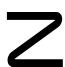
\includegraphics[keepaspectratio]{images/part001_3d6df7c1.jpg}}

因此，关系 \([M:L]=0\) 表示不存在同构于 L 的 M 的直因子子模。但这并不排除存在同构于 L 的 M 的子模；只需考虑例子 A=Z，L=Z/2Z，M=Z/4Z：Z-模 L 与 M 都是原始的且不同构，故 \([M:L]=0\)，而 L 同构于 M 的子模 \(2Z/4Z\)。

\subsection{有限长度模的结构}

定理 2（克鲁尔–雷马克–施密特）. —— 设 A 是一个环，M 是一个有限长度的 A-模。

\begin{enumerate}
\def\labelenumi{\alph{enumi})}
\item
  存在 M 的不可分解子模的一个有限族 \((\mathrm{M}_i)_{i\in \mathrm{I}}\)，使 \(\mathrm{M} = \bigoplus_{i\in \mathrm{I}}\mathrm{M}_i\)，且模 M 是半原始的。
\item
  设 \((\mathrm{M}_{i})_{i\in\mathrm{I}}\) 与 \((\mathrm{M}_{j}^{\prime})_{j\in\mathrm{J}}\) 是 M 的不可分解子模的两个有限族，使得 \(M=\bigoplus_{i\in I}M_{i}=\bigoplus_{j\in J}M_{j}^{\prime}\) 。存在从 I 到 J 的一个双射 \(\sigma\) 与 M 的一个自同构 u，使 \(u(\mathrm{M}_{i})=\mathrm{M}_{\sigma(i)}^{\prime}\) 对每个 \(i\in I\) 成立。
\item
  设 \(\mathrm{N}\) 是 \(\mathrm{M}\) 的一个直因子子模，并设 \((\mathrm{M}_i)_{i\in \mathrm{I}}\) 是 \(\mathrm{M}\) 的不可分解子模的一个有限族，其直和为 \(\mathrm{M}\) 。存在子集 \(\mathrm{J}\) ⊂ \(\mathrm{I}\)，使 \(\bigoplus_{i\in \mathrm{I - J}}\mathrm{M}_i\) 与 \(\mathrm{N}\) 互补。模 \(\mathrm{N}\) 同构于 \(\bigoplus_{j\in \mathrm{J}}\mathrm{M}_j\) 。
\item
  设 \(\mathbf{N}\) 是一个 A-模。若存在整数 \(d > 0\) 使模 \(\mathbf{M}^d\) 与 \(\mathbf{N}^d\) 同构，则模 \(\mathbf{M}\) 与 \(\mathbf{N}\) 同构。
\item
  设 \(\mathrm{N}\) 与 \(\mathrm{P}\) 是有限长度的 A-模。若模 \(\mathrm{M} \oplus \mathrm{P}\) 与 \(\mathrm{N} \oplus \mathrm{P}\) 同构，则 \(\mathrm{M}\) 与 \(\mathrm{N}\) 同构。
\end{enumerate}

有限长度的模既是阿廷的又是诺特的（VIII，第 2 页，命题 1）。此外，对有限长度的模而言，不可分解与原始是一回事（VIII，第 31 页，命题 4）。于是断言 a) 由 VIII，第 30 页的命题 3 得出。断言 b)、c)、e) 分别由 VIII，第 32 页定理 1 的推论 2、推论 5、推论 3 得出。最后，断言 d) 由 VIII，第 35 页的推论 4 得出，因为在 d) 的假设下，模 N 长度有限，从而由 a) 是半原始的。

定理 3. —— 设 K 是一个交换域，A 是一个 K-代数，M 与 N 是有限长度的模。设 \(K'\) 是一个非零交换 K-代数，使得 \(\mathrm{A}_{(\mathrm{K}')}\) -模 \(\mathrm{M}_{(\mathrm{K}')}\) 与 \(\mathrm{N}_{(\mathrm{K}')}\) 同构。则 A-模 M 与 N 同构。

\begin{enumerate}
\def\labelenumi{\alph{enumi})}
\item
  先设代数 \(K'\) 在 K 上具有有限次数 d。则 A-模 \(\mathrm{M}_{(\mathrm{K}')}\) 同构于 \(M^{d}\)，A-模 \(\mathrm{N}_{(\mathrm{K}')}\) 同构于 \(\mathbf{N}^d\)，故 A-模 \(\mathbf{M}^d\) 与 \(\mathbf{N}^d\) 同构。由定理 2, d)，A-模 \(\mathbf{M}\) 与 \(\mathbf{N}\) 同构。
\item
  现在设 K-代数 \(K'\) 由有限多个元素生成。取 \(K'\) 的一个极大理想 m，并令 \(K'' = K'/m\) 。由希尔伯特零点定理（VIII，第 462 页，定理 1 的推论 1），\(K''\) 是 K 的一个有限次扩张。把标量从 \(K'\) 扩张到 \(K''\) ，我们由 \(A_{(K')}\) -线性同构 \(M_{(K')} \to N_{(K')}\) 得到 \(A_{(K'')}\) -线性同构 \(M_{(K'')} \to N_{(K'')}\) 。由证明的 a)，A-模 M 与 N 同构。
\item
  最后处理一般情形。设 \(u: \mathrm{M}_{(\mathrm{K}')} \to \mathrm{N}_{(\mathrm{K}')}\) 是 \(\mathrm{A}_{(\mathrm{K}')}\) -模的一个同构，\(v: \mathrm{N}_{(\mathrm{K}')} \to \mathrm{M}_{(\mathrm{K}')}\) 是其逆同构。用 \(\mathcal{E}\) 表示由有限多个元素生成的 \(\mathrm{K}'\) 的 K-子代数组成的集合。若 E 是这样的一个子代数，则 \(\mathrm{A}_{(\mathrm{E})}\) 等同于 \(\mathrm{A}_{(\mathrm{K}')}\) 的一个子环，且 \(\mathrm{M}_{(\mathrm{E})}\) 与 \(\mathrm{N}_{(\mathrm{E})}\) 分别等同于 \(\mathrm{A}_{(\mathrm{E})}\) -子模——前者在 \(\mathrm{M}_{(\mathrm{K}')}\) 中，后者在 \(\mathrm{N}_{(\mathrm{K}')}\) 中（II, §7, No.~7, 第 306 页）；此外，\(\mathrm{M}_{(\mathrm{K}')}\) 与 \(\mathrm{N}_{(\mathrm{K}')}\) 分别是右有向族 \((\mathrm{M}_{(\mathrm{E})})_{\mathrm{E} \in \mathcal{E}}\) 与 \((\mathrm{N}_{(\mathrm{E})})_{\mathrm{E} \in \mathcal{E}}\) 的并。A-模 M 与 N 长度有限，从而是有限生成的；设 S 是 A-模 M 的一个有限生成元集，T 是 A-模 N 的一个有限生成元集。存在 K-代数 \(\mathrm{E} \in \mathcal{E}\)，使 \(u(1 \otimes s) \in \mathrm{N}_{(\mathrm{E})}\) 对每个 \(s \in \mathrm{S}\) 成立，且 \(v(1 \otimes t) \in \mathrm{M}_{(\mathrm{E})}\) 对每个 \(t \in \mathrm{T}\) 成立。由线性性推出 \(u(\mathrm{M}_{(\mathrm{E})}) \subset \mathrm{N}_{(\mathrm{E})}\) 与 \(v(\mathrm{N}_{(\mathrm{E})}) \subset \mathrm{M}_{(\mathrm{E})}\) 。于是映射 \(u\) 与 \(v\) 诱导出从 \(\mathrm{M}_{(\mathrm{E})}\) 到 \(\mathrm{N}_{(\mathrm{E})}\) 以及从 \(\mathrm{N}_{(\mathrm{E})}\) 到 \(\mathrm{M}_{(\mathrm{E})}\) 的互逆双射。这些双射显然是 \(\mathrm{A}_{(\mathrm{E})}\) -线性的。于是 \(\mathrm{A}_{(\mathrm{E})}\) -模 \(\mathrm{M}_{(\mathrm{E})}\) 与 \(\mathrm{N}_{(\mathrm{E})}\) 同构。由证明的 b)，A-模 M 与 N 同构。
\end{enumerate}

注. —— 设 E 与 F 是交换域 K 上的两个有限维向量空间，并设 \(K'\) 是 K 的一个扩张。设 u 是 E 的一个自同态，v 是 F 的一个自同态，并设经标量扩张得到的 \(u_{(K')}\) 与 \(v_{(K')}\) 是 \(E_{(K')}\) 与 \(F_{(K')}\) 的自同态。由 VII, §5, No.~3, 第 32 页的推论 1 与推论 2，自同态 u 与 v 相似当且仅当自同态 \(u_{(K')}\) 与 \(v_{(K')}\) 相似。这一点也可由把上面的定理 3 应用于代数 A = K{[}X{]} 及 A-模 \(M = E_u\) 与 \(N = F_v\)（VII, §5, No.~1, 第 29 页）而得到。

\BourbakiExercises{习题}

\begin{enumerate}
\def\labelenumi{\arabic{enumi})}
\tightlist
\item
  \begin{enumerate}
  \def\labelenumii{\alph{enumii})}
  \tightlist
  \item
    给出一个诺特模 M 的例子，使得 M 的每个非零自同态都是单射，并且存在 M 的非零且非双射的自同态。
  \end{enumerate}
\end{enumerate}

\begin{enumerate}
\def\labelenumi{\alph{enumi})}
\setcounter{enumi}{1}
\tightlist
\item
  给出一个阿廷模 M 的例子，使得 M 的每个非零自同态都是满射，并且存在 M 的非零且非双射的自同态。
\end{enumerate}

\begin{enumerate}
\def\labelenumi{\arabic{enumi})}
\setcounter{enumi}{1}
\item
  设 \(\mathrm{A}\) 是一个环，其中双边理想的每个递增序列 \((\mathfrak{a}_n)_{n\in \mathbf{N}}\) 都是平稳的（例如，左或右诺特环）。证明环 \(\mathrm{A}\) 的每个满射自同态都是双射。
\item
  给出一个环的例子，它有两个元素 u、v，使得 uv = 1 且 \(vu \neq 1\)。证明这样的环不是诺特子环的一个有向族的并。
\item
  设 M 是一个 A-模，p 与 q 是 M 的两个投影算子。
\end{enumerate}

\begin{enumerate}
\def\labelenumi{\alph{enumi})}
\item
  我们有 \(p(\mathrm{M}) \subset q(\mathrm{M})\) 当且仅当 qp = p；核 \(\operatorname{Ker}(p)\) 包含于 \(\operatorname{Ker}(q)\) 当且仅当 qp = q。
\item
  和 \(p + q\) 是投影算子当且仅当 pq = -qp。若 \(p + q\) 是投影算子，且在 M 中关系 2x = 0 蕴含 x = 0，则我们有 pq = 0 与 qp = 0。
\item
  证明下列性质等价：
\end{enumerate}

\begin{enumerate}
\def\labelenumi{(\roman{enumi})}
\item
  我们有 \(pq = qp\)。
\item
  我们有 \(q(p(\mathbb{M})) \subset p(\mathbb{M})\) 与 \(q(\operatorname{Ker}(p)) \subset \operatorname{Ker}(p)\) 。
\item
  存在 M 的两两正交的投影算子的序列 \((p_1, p_2, p_3, p_4)\)，使得 \(p = p_1 + p_2\)、\(q = p_1 + p_3\)，且 \(1_{\mathrm{M}} = p_1 + p_2 + p_3 + p_4\) 。
\end{enumerate}

这样的序列（当它存在时）是唯一的：我们有 \(p_{1} = pq\) 。

\begin{enumerate}
\def\labelenumi{\arabic{enumi})}
\setcounter{enumi}{4}
\tightlist
\item
  设 \(\mathrm{A}\) 是一个环。
\end{enumerate}

\begin{enumerate}
\def\labelenumi{\alph{enumi})}
\item
  A 的元素 e 是幂等的当且仅当映射 \(x \mapsto xe\) 是左 A-模 \(A_{s}\) 的一个投影算子（相应地，映射 \(x \mapsto ex\) 是右 A-模 \(A_{d}\) 的一个投影算子）。
\item
  设 \(e_{1}, e_{2}\) 是环 A 中的幂等元。证明群 \(\mathrm{Hom}_{\mathrm{A}}(\mathrm{Ae}_{1}, \mathrm{Ae}_{2})\) 同构于 \(e_{1}A \cap Ae_{2} = e_{1}Ae_{2}\)，且环 \(\mathrm{End}_{\mathrm{A}}(\mathrm{Ae}_{1})\) 同构于环 \(e_{1}Ae_{1}\) 。
\item
  设 \(e_1, e_2\) 是 A 中的幂等元。证明下列性质等价：
\end{enumerate}

\begin{enumerate}
\def\labelenumi{(\roman{enumi})}
\item
  \(Ae_{1} = Ae_{2}.\)
\item
  \(e_{1}e_{2}=e_{1}\) 与 \(e_{2}e_{1}=e_{2}\) 。
\item
  \((1 - e_{1})\mathrm{A} = (1 - e_{2})\mathrm{A}.\)
\end{enumerate}

当这些性质成立时，存在可逆元 \(a \in \mathrm{A}\)，使 \(e_2 = ae_1a^{-1}\) 。

\begin{enumerate}
\def\labelenumi{\alph{enumi})}
\setcounter{enumi}{3}
\tightlist
\item
  设 \(e_{1}, e_{2}\) 是 A 中的两个幂等元。证明下列性质等价：
\end{enumerate}

\begin{enumerate}
\def\labelenumi{(\roman{enumi})}
\item
  左 A-模 \(Ae_{1}\) 与 \(Ae_{2}\) 同构。
\item
  右 A-模 \(e_1\mathrm{A}\) 与 \(e_2\mathrm{A}\) 同构。
\item
  存在元素 \(x, y\) 属于 \(A\)，使得 \(xy = e_1\) 且 \(yx = e_2\) 。
\end{enumerate}

当这些性质成立时，我们称 \(e_{1}\) 与 \(e_{2}\) 是等价幂等元。

\begin{enumerate}
\def\labelenumi{\alph{enumi})}
\setcounter{enumi}{4}
\tightlist
\item
  若 A 中的幂等元等价且属于 A 的中心，则它们相等。
\end{enumerate}

\(f\) ) 设 \((e_i)_{i\in \mathrm{I}}\) 与 \((f_{i})_{i\in \mathrm{I}}\) 是 A 中幂等元的有限族，使得 \(e_i e_j = 0\) 与 \(f_{i} f_{j} = 0\)（对 \(i\in \mathrm{I}, j\in \mathrm{I}, i\neq j\)），且 \(e_i\) 等价于 \(f_{i}\)（对每个 \(i\in \mathrm{I}\)）。则 \(e = \sum_{i\in \mathrm{I}}e_i\) 与 \(f = \sum_{i\in \mathrm{I}}f_{i}\) 是 A 中的等价幂等元。

¶ 6) 设 A 是环，u 与 v 是 A 的两个元素，使得 uv = 1 且 vu ≠ 1。对 i ≥ 1 与 j ≥ 1，令 \(e_{ij} = v^{i-1}u^{j-1} - v^i u^j\) 。

\begin{enumerate}
\def\labelenumi{\alph{enumi})}
\item
  证明我们有 \(e_{ij} \neq 0\) 与 \(e_{ij}e_{hk} = \delta_{jh}e_{ik}\)，其中 \(i,j,k,h\) 为整数 \(\geqslant 1\) 。
\item
  证明 A 的左理想 \(Ae_{ii}\)（对 \(i \geqslant 1\)）都非零、作为 A-模两两同构（利用习题 5 d)），且它们的和是直和。
\item
  证明我们有 \(u(v + e_{1i}) = 1\)（对每个 \(i \geqslant 1\)），且 \(e_{1i} \neq e_{1j}\)（对 \(i \geqslant 1, j \geqslant 1, i \neq j\)）。
\item
  设 B 是一个环，它具有 VIII，第 15 页习题 7 a) 的诸等价性质。由上题推出：B 的每个左可逆或右可逆的元素都是可逆的。
\end{enumerate}

\begin{enumerate}
\def\labelenumi{\arabic{enumi})}
\setcounter{enumi}{6}
\tightlist
\item
  用 A（相应地 a）表示形如 \(\mathrm{P}/(\mathrm{X}^{2}+1)^{n}\) 的有理分式组成的集合，其中 n 是整数 \(\geqslant0\)，\(P\in \mathbf{Q}[X]\) 是次数 \(\leqslant2n\)（相应地 \(\leqslant2n-1\)）的多项式。a) 证明 A 是体 \(\mathbf{Q}(X)\) 的一个子环，且 a 是环 A 的一个理想。b) A-模 \(a\oplus a\) 与 \(A\oplus A\) 同构。A-模 a 是投射的且有限生成的，但不同构于 A。
\end{enumerate}

\begin{enumerate}
\def\labelenumi{\alph{enumi})}
\setcounter{enumi}{2}
\tightlist
\item
  存在 \(\mathbf{K}\)，它是体 \(\mathbf{Q}\) 的一个二次扩张，使得 \(\mathrm{A}_{(\mathrm{K})}\) -模 \(\mathfrak{a}_{(\mathrm{K})}\) 与 \(\mathrm{A}_{(\mathrm{K})}\) 同构。
\end{enumerate}

\begin{enumerate}
\def\labelenumi{\arabic{enumi})}
\setcounter{enumi}{7}
\item
  设 A 是一个左阿廷环，并设 M 与 N 是 A-模 \(A_{s}^{n}\) 中两个互补的子模。若 M 是自由 A-模，则 N 是自由 A-模。
\item
  设 A 是一个完备拓扑环，m 是 A 的一个双边理想。假设环 A/m 是体，m 的每个元素都拓扑幂零（Gen.~Top., III, §6, 第 317 页，习题 9），且存在由 A 的加法群的子群组成的、A 中 0 的邻域的基本系。则环 A 是局部环，且 m 是其极大理想。特别地，对每个素数 p，p 进整数环 \(\mathbf{Z}_{p}\)（V, §12, No.~3, 第 96 页）是局部的，其极大理想是 \(p\mathbf{Z}_{p}\) 。
\end{enumerate}

¶ 10) 设 p 是素数，q 是 p 的幂，G 是 q 阶有限群，A 是交换环。设 \((e_{g})\) 是 A 上群 G 的代数 A{[}G{]} 的典范基。

\begin{enumerate}
\def\labelenumi{\alph{enumi})}
\item
  把 \(\mathfrak{a}\) 定义为元素 \(\sum a_{g}e_{g}\)（A{[}G{]} 中满足 \(\sum a_{g} = 0\) 者）组成的集合，它是 A{[}G{]} 的一个双边理想。若环 A 的特征为 \(p\)（V, §1, No.~2, 第 2 页），则我们有 \(x^{q} = 0\) 对每个 \(x\in \mathfrak{a}\) 成立（对 \(q\) 用归纳法；若 \(q\neq 1\)，取 G 的中心中一个元素 \(h\)，其阶为 \(p\)（I, §6, No.~5, 第 77 页，命题 11 的推论），并由归纳假设推出存在 \(y\in \mathrm{A}[\mathrm{G}]\) 使 \(x^{q / p} = (1 - e_h)y\)）。
\item
  设 A 是局部环，其极大理想为 m，且体 A/m 的特征为 p。证明环 A{[}G{]} 是局部环，且其极大理想是元素 \(\sum a_{g}e_{g}\in A[G]\)（满足 \(\sum a_{g}\in m\)）组成的集合。
\end{enumerate}

（设 S 是一个单 A{[}G{]}-模；证明 S 被 m 零化，然后，把 I, §6, No.~5, 第 76 页的命题 11 应用于由 S 的一个非零元素生成的 Z{[}G{]}-子模，证明 S 含有一个在 G 下不变的元素。）

\begin{enumerate}
\def\labelenumi{\arabic{enumi})}
\setcounter{enumi}{10}
\tightlist
\item
  设 p 是素数，G 是一个不含 p 阶元素的群，A 是一个不含非零幂零元素的、特征为 p 的交换环，A{[}G{]} 是 G 在 A 上的代数，\((e_{g})\) 是 A{[}G{]} 在 A 上的典范基。证明环 A{[}G{]} 没有非零的诣零理想（注意：若元素 \(\sum a_{g}e_{g} \in A[G]\) 幂零，则我们有 \(a_{1} = 0\)）。
\end{enumerate}

¶ 12) 设 K 是交换域，E 与 F 是 K 的扩张，A 是环 \(E \otimes_{K} F\) 。

\begin{enumerate}
\def\labelenumi{\alph{enumi})}
\tightlist
\item
  若 E 与 F 是 K 的超越扩张，则环 A 不是局部环。b) 设 E 是 K 的一个代数扩张，并用 \(E_{s}\) 与 \(F_{s}\) 分别表示 K 在 E 与 F 中的可分闭包。下列性质等价：
\end{enumerate}

\begin{enumerate}
\def\labelenumi{(\roman{enumi})}
\item
  环 A 是局部环。
\item
  环 \(\mathrm{E}\otimes_{\mathrm{K}}\mathrm{F}_s\) 是整环。
\item
  环 \(E \otimes_{K} F_{s}\) 是体。
\item
  环 \(E_{s} \otimes_{K} F_{s}\) 是体。
\end{enumerate}

当这些性质成立时，A 的极大理想 \(\mathfrak{m}\) 是 A 的幂零元素组成的集合，且 E 与 F 的每个复合扩张都同构于 \(A / \mathfrak{m}\) 。

\begin{enumerate}
\def\labelenumi{\arabic{enumi})}
\setcounter{enumi}{12}
\item
  设 A 是一个不是体的局部整环（例如 \(\mathbf{Z}_{(p)}\)，参见 VIII，第 26 页，例 5），并设 a 是 A 的一个非零不可逆元。把 A-模 \(\mathrm{A}^{(\mathbf{N})}\) 记作 M，其典范基记作 \((e_{n})_{n\in\mathbf{N}}\)。证明序列 \((f_{n})_{n\in\mathbf{N}}\)——其中 \(f_{2m}=e_{2m}\) 与 \(f_{2m+1}=e_{2m+1}+ae_{2m+2}\)（对每个 \(m\geqslant0\)）——是 M 在 A 上的一个基。证明 M 的子模 \(N=\sum_{m\geqslant0}\mathrm{A}(e_{2m}+ae_{2m+1})\) 是直因子，但不存在 N 的子集 J 使 \(\sum_{n\in J}Af_{j}\) 与 N 互补。由此推出：在 VIII，第 35 页的推论 5 中，不能略去 I 有限的假设。
\item
  设 A 是环，M 是 A-模，N 是 M 的一个原始直因子。设 \(M = \bigoplus_{i \in I} M_i\) 是 M 的一个直和分解，\((p_i)_{i \in I}\) 是相伴的投影算子族。证明存在 \(i \in I\)，使 \(p_i\) 诱导出从 N 到 \(M_i\) 的一个直因子的同构。
\item
  设 A 是环，并设 M、N、P 是 A-模。若模 \(M \oplus P\) 与 \(N \oplus P\) 同构且模 P 是原始的，则模 M 与 N 同构。
\item
  设 A 是环，M 是一个有限长度的 A-模，\((\mathrm{M}_{i})_{i\in\mathrm{I}}\) 是以 M 为直和的 M 的不可分解子模族。设 L 是一个有限长度的不可分解 A-模，\(I_{L}\) 是指标 \(i\in I\) 中使 \(M_{i}\) 同构于 L 的那些指标的集合。用例子说明 M 的子模 \(\sum_{i\in I_{L}}M_{i}\) 未必在 M 的自同构下稳定。
\item
  设 \(\mathrm{A}\) 是环，\(n\) 是整数，\(X \in \mathbf{GL}_n(\mathrm{A})\) 。
\end{enumerate}

\begin{enumerate}
\def\labelenumi{\alph{enumi})}
\item
  设环 A 是局部环。证明存在 \(\mathbf{GL}_{n}(\mathrm{A})\) 中的矩阵 P、Q，它们是形如 \(B_{ij}(\lambda)\) 的矩阵（II, §10, No.~13, 第 361 页）的乘积，以及 A 的一个可逆元 \(\delta\)，使得我们有 \(PXQ = \text{diag}(1, \ldots, 1, \delta)\)（照出处同前中命题 14 的证明进行）。
\item
  设环 A 是欧几里得环（VII, §1, 第 49 页，习题 7）。证明同样的结果。
\item
  若 \(\mathrm{A}\) 是局部环或欧几里得交换环，则群 \(\mathbf{S}\mathbf{L}_n(\mathbf{A})\) 由矩阵 \(B_{ij}(\lambda)\) 生成。
\item
  设 A 是局部环，其极大理想记作 m。证明 \(\mathbf{M}_{n}(\mathrm{A})\) 中每个在 \(\mathbf{M}_{n}(\mathrm{A}/\mathfrak{m})\) 中的像可逆的矩阵本身可逆（利用 II, §10, No.~13, 第 361 页的引理 1）。
\end{enumerate}

\begin{enumerate}
\def\labelenumi{\arabic{enumi})}
\setcounter{enumi}{17}
\tightlist
\item
  设 A 是局部环，E 是自由 A-模，x 是 E 的一个非零元素。设 \((e_{i})_{i\in I}\) 是 E 的一个使 x 的非零坐标个数尽可能少的基。设 \(x=\sum a_{i}e_{i}\) 是 x 在此基下的表示；用 J 表示指标 \(i\in I\) 中使 \(a_{i}\neq0\) 的那些指标的集合。
\end{enumerate}

\begin{enumerate}
\def\labelenumi{\alph{enumi})}
\tightlist
\item
  证明诸 \(a_{i}\) 中没有一个属于由其余元素生成的 A 的右理想。
\item
  设 F 与 G 是 E 的两个互补的子模，使得 \(x \in F\)；对 \(i \in I\)，写 \(e_{i} = f_{i} + g_{i}\)，其中 \(f_{i} \in F\)、\(g_{i} \in G\)。证明由 \(f_{j}\)（\(j \in J\)）与 \(e_{i}\)（\(i \in I - J\)）组成的族是 E 的一个基（若 \(g_{j} = \sum_{k \in I} b_{jk} e_{k}\)，注意 j、k 属于 J 时坐标 \(b_{jk}\) 属于 A 的极大理想，并应用习题 17 d)）。由此推出：存在 F 的一个自由子模，它包含 x 且是 F 的直因子。
\end{enumerate}

\(c\) ) 证明每个投射 A-模都是自由的（利用 Kaplansky 定理（II, §2, 第 386 页，习题 2）化为具有可数生成元族的模的情形，并应用 \(b\)））。

\begin{enumerate}
\def\labelenumi{\arabic{enumi})}
\setcounter{enumi}{18}
\item
  设 A 是交换环，M 是有限生成 A-模，u 是 M 的一个自同构，N 是 M 的一个在 u 下稳定的子模。证明我们有 \(u(N) = N\)（利用 VIII，第 28 页的推论 1, d)）。
\item
  设 A 是环，M 是一个有限长度的 A-模，N 是一个 A-模。设 m 与 n 是严格正整数，使得 \(M^{m}\) 与 \(N^{n}\) 同构。证明存在 A-模 P 与整数 p、q，使得 M 同构于 \(P^{p}\)，N 同构于 \(P^{q}\)，且 mp = nq。
\end{enumerate}

\section{单模}

\subsection{单模}

回忆下面的定义（II, §1, No.~10, 第 212 页）。

定义 1. —— 设 A 是环。若一个 A-模 M 非零且没有异于 0 与 M 的子模，则称它为单模。

A-模 M 是单模当且仅当 M 是其位似环 \(A_{M}\) 上的单模。每个单模都不可分解、长度为 1，从而是原始模（VIII，第 31 页，命题 4, b)）。

例. —— 1) 模 \(A_{s}\) 是单 A-模当且仅当 A 是体（I, §9, No.~1, 第 115 页，定理 1）。这时单 A-模就是体 A 上的 1 维向量空间。

\begin{enumerate}
\def\labelenumi{\arabic{enumi})}
\setcounter{enumi}{1}
\item
  设 A 是一个主理想整环（VII, §1, No.~1, 第 1 页，定义 1）且不是体。对 A 的每个不可约元 \(\pi\)，A-模 \(A_s / (\pi)\) 都是单模，且每个单 A-模都同构于这样一个模（VII, §4, No.~8, 第 25 页，注 4）。对 \(n \geqslant 2\)，A-模 \(A_s / (\pi^n)\) 不可分解（VII, §4, No.~8, 第 24 页，命题 8）但不是单模。
\item
  设 K 是体，V 是体 K 上的一个非零右向量空间，A 是环 \(\operatorname{End}_{\mathrm{K}}(\mathrm{V})\) 的一个包含 V 的有限秩自同态的子环（例如 \(\mathrm{A} = \operatorname{End}_{\mathrm{K}}(\mathrm{V})\)）。我们来证明 V 是单 A-模：设 W 是 V 的一个非零 A-子模，x 是 W 的一个非零元素；存在 V 上的一个线性型 \(\varphi\)，使 \(\varphi(x) \neq 0\)（II, §7, No.~5, 第 300 页，定理 6）。对 V 中每个 y，映射 \(z \mapsto y\varphi(z)\)——它是秩 \(\leqslant 1\) 的线性映射——属于 A；于是我们有 Ax = V，从而更有 W = V，这证明 V 是单 A-模。
\end{enumerate}

命题 1. —— 设 A 是环。

\begin{enumerate}
\def\labelenumi{\alph{enumi})}
\item
  设 \(\mathfrak{m}\) 是 A 的一个左理想。A-模 \(\mathrm{A}_s / \mathfrak{m}\) 是单模当且仅当 \(\mathfrak{m}\) 是极大左理想。
\item
  设 M 是单 A-模，x 是 M 的一个非零元素。我们有等式 \(M = Ax\)，x 的零化子 m 是 A 的一个极大左理想，且映射 \(a \mapsto ax\) 通过过渡到商定义出从 \(A_{s}/m\) 到 M 的一个同构。
\item
  设 M 是一个非零 A-模。若对 M 的每个非零元素 x 都有 M = Ax，则 M 是单模。
\end{enumerate}

\(A_{s}/m\) 的子模都具有形式 n/m，其中 n 是 A 的包含 m 的左理想（I, §4, No.~6, 第 41 页，定理 4）；因此，A-模 \(A_{s}/m\) 是单模当且仅当我们有 \(m \neq A\)，且 A 的每个包含 m 的左理想 n 都满足 n/m = 0 或 \(n/m = A_{s}/m\)，即 n = m 或 n = A。这就证明了 a)。

在 b) 的假设下，Ax 是 M 的一个非零子模，从而等于 M。于是，映射 \(a \mapsto ax\) 通过过渡到商定义出从 \(A_{s}/m\) 到 M 的一个同构；因此 A-模 \(A_{s}/m\) 是单模，且由 a) 左理想 m 是极大的。这就证明了 b)。

在 c) 的假设下，设 N 是 M 的一个非零子模。若 x 是 N 的一个非零元素，则我们有 \(Ax \subset N\) 且 Ax = M，从而 M = N。于是 M 是单模。

推论 1. —— 若环 A 不化为 0，则存在单 A-模。

事实上，由克鲁尔定理（I, §8, No.~6, 第 104 页，定理 1），A 存在极大左理想。

推论 2. —— 设 A 是一个局部环（VIII，第 26 页，定义 1），r 是其极大理想。A-模 \(A_{s}/r\) 是单模，且每个单 A-模都同构于 \(A_{s}/r\) 。

注. —— 1) 设 A 是交换环，m 是 A 的一个理想。则 m 是 A-模 \(A_{s}/m\) 的零化子（II, §1, No.~12, 第 219 页，定义 11）。因此，若 m 与 \(m'\) 是 A 的不同理想，则 A-模 \(A_{s}/m\) 与 \(A_{s}/m'\) 不同构。存在忠实单 A-模（II, §1, No.~12, 第 219 页）当且仅当 (0) 是 A 的极大理想，即 A 是体。

\begin{enumerate}
\def\labelenumi{\arabic{enumi})}
\setcounter{enumi}{1}
\tightlist
\item
  我们可以给出一个非交换环 A 及其两个不同的极大左理想 m 与 \(m'\) 的例子，使得 A-模 \(A_{s}/m\) 与 \(A_{s}/m'\) 同构（VIII，第 52 页，习题 3）。
\end{enumerate}

\subsection{舒尔引理}

命题 2. —— 设 A 是环，M 与 N 是两个 A-模，f 是从 M 到 N 的一个非零同态。

\begin{enumerate}
\def\labelenumi{\alph{enumi})}
\item
  若 M 是单模，则 f 是单射。
\item
  若 \(\mathbf{N}\) 是单模，则 \(f\) 是满射。
\item
  若 M 与 N 都是单模，则 f 是同构。
\end{enumerate}

f 的核是 M 的真子模，f 的像是 N 的非零子模。

\begin{enumerate}
\def\labelenumi{\alph{enumi})}
\item
  若 M 是单模，则我们有 \(\operatorname{Ker}(f)=0\)，故 f 是单射。
\item
  若 \(N\) 是单模，则我们有 \(\operatorname{Im}(f) = N\)，故 \(f\) 是满射。
\item
  若 M 与 N 都是单模，则 f 既单又满。
\end{enumerate}

推论（舒尔引理）. —— 单模的自同态环是体。

若 M 是单 A-模，则非零环 \(\operatorname{End}_{\mathrm{A}}(\mathrm{M})\) 的每个非零元素都可逆（命题 2, c)），故 \(\operatorname{End}_{\mathrm{A}}(\mathrm{M})\) 是体。

定理 1. —— 设 K 是一个代数闭交换域，A 是一个 K-代数，M 是一个单 A-模。假设 M 作为 K 上向量空间的维数有限，或更一般地，严格小于 K 的基数。则 A-模 M 的自同态环由位似 \(\alpha_{M}\)（\(\alpha \in K\)）组成。

设 \(\mathrm{E}\) 是 A-模 \(\mathrm{M}\) 的自同态环；由命题 2 的推论它是体，且是体 \(\mathrm{K}\) 上的一个代数。若把 \(\mathrm{M}\) 看作体 \(\mathrm{E}\) 上的左向量空间，则由 II, §1, No.~13, 第 222 页的命题 25，我们有 \(\dim_{\mathrm{K}} \mathrm{M} = (\dim_{\mathrm{E}} \mathrm{M})[\mathrm{E} : \mathrm{K}]\)，从而 \(\dim_{\mathrm{K}} \mathrm{M} \geqslant [\mathrm{E} : \mathrm{K}]\) 。由于按假设 \(\dim_{\mathrm{K}} \mathrm{M} < \operatorname{Card}(\mathrm{K})\)，等式 \(\mathrm{E} = \mathrm{K} \cdot 1_{\mathrm{M}}\) 便是下面引理的推论。

引理 1. —— 设 E 是体，K 是 E 的中心的一个不等于 E 的子体。若体 K 是代数闭的，则我们有 \([E:K] \geqslant \text{Card}(K)\) 。

设 \(x\) 是 \(\mathrm{E} - \mathrm{K}\) 的一个元素，\(\mathrm{L}\) 是 \(\mathrm{E}\) 的由 \(\mathrm{K} \cup \{x\}\) 生成的（交换）子体。由于 \(\mathrm{K}\) 是代数闭的，\(x\) 在 \(\mathrm{K}\) 上是超越的。由 VII, §2, No.~3, 第 10 页定理 2 及第 11 页，元素 \((x - \alpha)^{-1}\)（属于 \(\mathrm{L}\)，其中 \(\alpha\) 取遍 \(\mathrm{K}\)）在 \(\mathrm{K}\) 上线性无关。因此我们有 \([\mathrm{E} : \mathrm{K}] \geqslant [\mathrm{L} : \mathrm{K}] \geqslant \operatorname{Card}(\mathrm{K})\) 。

例. —— *设 A 是一个由可数族元素生成的 C-代数；它在 C 上有可数维。设 M 是一个单 A-模；

它是单生成的，故在 \(\mathbf{C}\) 上具有可数基。由于体 \(\mathbf{C}\) 不是可数的（Gen.~Top., IV, §4, No.~1, 第 44 页），我们有 \([\mathrm{M}:\mathbf{C}] < \mathrm{Card}(\mathbf{C})\) 。因此 A-模 M 的自同态就是位似 \(\alpha_{\mathrm{M}}\)（\(\alpha \in \mathbf{C}\)）。这特别适用于 A 是 \(\mathbf{C}\) 上有限维李代数的泛包络代数的情形（Lie, I, §2, No.~7, 第 21 页，推论 3）。*

推论 1. —— 保留定理 1 的假设，并再设代数 A 是交换的。则 M 在 K 上的维数为 1。

由于环 A 交换，\(a_{M}\) 对每个 \(a \in A\) 都是 A-模 M 的自同态。于是由定理 1，我们有 \(A_{M} = K \cdot 1_{M}\)，且 M 是单 K-模，即体 K 上的 1 维向量空间。

推论 2. —— 设 K 是交换域，A 是一个 K-代数，M 是一个 A-模。假设对 K 的每个扩张 L，\(\mathrm{A}_{(\mathrm{L})}\) -模 \(\mathrm{M}_{(\mathrm{L})}\) 都是单模。则 M 的自同态环由位似 \(\alpha_{M}\)（\(\alpha \in K\)）组成。

设 I 是一个基数严格大于 M 在 K 上的维数的集合（例如 M 的子集组成的集合）。设 L 是体 \(\mathrm{K}((\mathrm{X}_{i})_{i\in\mathrm{I}})\) 的一个代数闭包（V, §4, No.~3, 第 23 页，定理 2）。取 L 上的一个 K-线性型 \(\varphi\)，使 \(\varphi(1)=1\)，并设 \(v:M_{(\mathrm{L})}\to M\) 是由 \(v(\alpha\otimes m)=\varphi(\alpha)m\) 刻画的 K-线性映射。设 u 是 M 的一个自同态。\(M_{(\mathrm{L})}\) 在 L 上的维数等于 M 在 K 上的维数，且严格小于 L 的基数。由定理 1，\(1_{L}\otimes u\)——\(A_{(\mathrm{L})}\) -模 \(M_{(\mathrm{L})}\) 的自同态——形如 \(\lambda\otimes1_{M}\)（\(\lambda\in L\)）。对每个 \(x\in M\)，我们有

\[
\begin{array}{c} u (x) = v \bigl (1 \otimes u (x) \bigr) = v \bigl ((1 _ {\mathrm{L}} \otimes u) (1 \otimes x) \bigr) \\ = v \bigl ((\lambda \otimes 1 _ {\mathrm{M}}) (1 \otimes x) \bigr) = v (\lambda \otimes x) = \varphi (\lambda) x, \end{array}
\]

于是 u 是位似 \(\varphi(\lambda)_{\mathrm{M}}\) 。

\subsection{极大子模}

定义 2. —— 设 A 是环，M 是一个 A-模。M 的极大子模就是 M 的真子模组成的集合（按包含关系排序）中的一个极大元。

\(A_{s}\) 的极大子模只不过是 A 的极大左理想。

设 N 是 M 的一个子模。M/N 的子模都具有形式 P/N，其中 P 是 M 的包含 N 的子模（I, §4, No.~6, 第 41 页，定理 4）。因此，N 是 M 的极大子模当且仅当模 M/N 是单模。

命题 3. —— 设 M 是一个有限生成 A-模。M 的每个真子模都包含在某个极大子模中。

设 N 是 M 的一个真子模。用 S 表示 M 的包含 N 的真子模组成的集合，按包含关系排序；我们来证明 S 是归纳的。设 F 是 S 的一个全序子集。若 F 为空，则 N 是 F 在 S 中的上界。在相反的情形，用 Q 表示 F 的诸元素之并。则 Q 是 M 的一个子模。设 F 是 M 的一个有限生成子集。若 Q 等于 M，则 F 将包含于某个子模 \(P \in F\)，这将蕴含 P = M，与 F 的定义矛盾。于是我们有 \(Q \in S\)，这证明 S 是归纳的。命题 3 于是由《集合论》，III, §2, No.~4, 第 155 页的推论 1 得出。

推论 1. —— 设 M 是一个非零的有限生成 A-模。存在 A 的一个双边理想 a——某个单 A-模的零化子——使得 aM 不等于 M。

设 N 是 M 的一个极大子模（命题 3），a 是单 A-模 M/N 的零化子；它是 A 的一个双边理想，且我们有 \(\mathfrak{a}(M/N)=0\)，由此 \(aM\subset N\)，从而 \(aM\neq M\) 。

推论 2. —— 设 A 是交换环，B 是一个 A-代数。设 M 是一个作为 A-模为有限生成的单 B-模，m 是 A-模 M 的零化子。则 m 是 A 的极大理想，且 M 是体 A/m 上的有限维向量空间。

由于环 A 交换，单 A-模的零化子是 A 的极大理想（VIII，第 46 页，命题 1）。把推论 1 应用于 A-模 M，存在 A 的一个极大理想 a，使 \(aM \neq M\) 。但 aM 是单 B-模 M 的一个子模；于是我们有 aM = 0，从而 \(a \subset m\) 。由于理想 m 异于 A，它等于 a，故 m 是极大的。模 M 是体 A/m 上的有限生成模；最后的断言由此得出。

\subsection{阿廷环上的单模}

设 A 是环。约定俗成地，若左理想 \(\alpha\) 是 A 的非零左理想组成的集合（按包含关系排序）中的一个极小元，我们就称它为 A 的极小左理想。右极小理想与双边极小理想类似地定义。

设 \(\mathfrak{a}\) 是 A 的一个左理想。则 \(\mathfrak{a}\) 是单 A-模当且仅当它是 A 的极小左理想。

左阿廷环（VIII，第 1 页，定义 1）的每个非零左理想都包含一个极小左理想。

命题 4. —— 设 A 是一个具有极小左理想 a 的环。每个忠实单 A-模都同构于 A-模 a。

设 M 是一个忠实单 A-模。设 \(\alpha\) 是 a 的一个非零元素。由于 A-模 M 是忠实的，存在 M 的一个元素 x，使 \(\alpha x \neq 0\) 。于是从 a 到 M 的同态 \(a \mapsto ax\) 非零；从而由 VIII，第 47 页的命题 2，它是同构。

命题 5. —— 设 A 是一个左阿廷环，M 是一个忠实 A-模。

\begin{enumerate}
\def\labelenumi{\alph{enumi})}
\item
  存在一个自然数 \(m\) 与一个从 \(\mathbf{A}_s\) 到 \(\mathbf{M}^m\) 的一个子模的同构。
\item
  若 M 有一个若尔当–赫尔德列 \((\mathrm{M}_{i})_{0\leqslant i\leqslant n}\)，则每个单 A-模都同构于诸商 \(M_{i}/M_{i+1}\) 之一。
\end{enumerate}

把 VIII，第 2 页应用于 A-模 \(A_{s}\) 与 M 的元素的零化子，存在 M 的元素 \(x_{1},\ldots,x_{m}\)，使 M 的零化子是诸 \(x_{i}\) 的零化子之交。由于 A-模 M 是忠实的，A-线性映射 \(a\mapsto(ax_{1},\ldots,ax_{m})\)（从 \(A_{s}\) 到 \(M^{m}\)）是单射，由此得 a)。

在 b) 的假设下，\(A_{s}\) 的每个单商都同构于 \(M^{m}\) 的某个若尔当–赫尔德列的一个商（I, §4, No.~7, 第 43 页，推论），从而同构于诸模 \(M_{i}/M_{i+1}\) 之一（I, §4, No.~7, 第 43 页，定理 6）。我们断定每个单 A-模都同构于 \(A_{s}\) 的一个商。

注. —— 命题 5 特别适用于下面两种情形：

\begin{enumerate}
\def\labelenumi{\alph{enumi})}
\item
  设 A 是交换域 K 上的一个代数，M 是 K 上的一个忠实的有限维模。则 M 是有限长度的 A-模，且 M 的反模是有限生成的。环 A 是左阿廷环（VIII，第 9 页，命题 6）。存在 A-模 M 的一个若尔当–赫尔德列 \((\mathrm{M}_{i})_{0\leqslant i\leqslant n}\)，且每个单 A-模都同构于诸模 \(M_{i}/M_{i+1}\)（对 \(0\leqslant i\leqslant n-1\)）之一。
\item
  设 A 是一个左阿廷环。模 \(A_{s}\) 长度有限（VIII，第 6 页，定理 1）。由于 A-模 \(A_{s}\) 长度有限，存在 A 的左理想的一个递减序列 \((\mathfrak{a}_{i})_{0\leqslant i\leqslant n}\)，使得 \(a_{0}=A\)、\(a_{n}=0\)，且 A-模 \(S_{i}=\mathfrak{a}_{i-1}/\mathfrak{a}_{i}\)（对 \(1\leqslant i\leqslant n\)）都是单模。则每个单 A-模都同构于诸模 \(S_{1},\ldots,S_{n}\) 之一。
\end{enumerate}

\subsection{单模的类}

用 \(\mathrm{Is}_{\mathrm{A}}\{\mathrm{X},\mathrm{Y}\}\) 表示关系

``A 是环且 X、Y 是同构的 A-模。''

这是关于 X 与 Y 的一个等价关系。若 X 是一个 A-模，则我们把对于 \(\operatorname{Is}_{\mathrm{A}}\) 与 X 等价的对象组成的类记作 \(\operatorname{cl}(\mathrm{X})\)，并称之为 A-模 X 的类（《集合论》，II, §6, No.~9, 第 122 页）。按定义，\(\operatorname{cl}(\mathrm{X})\) 是一个同构于 X 的 A-模；此外，两个 A-模 X 与 Y 同构当且仅当我们有 \(\operatorname{cl}(\mathrm{X}) = \operatorname{cl}(\mathrm{Y})\) 。

设 A 是环。关系

``\(\lambda\) 是一个有限生成 A-模的类''

在 \(\lambda\) 中是集合化的（《集合论》，II, §1, No.~4, 第 68 页）。事实上，每个有限生成 A-模都同构于形如 \(A_{s}^{n}/R\) 的 A-模，其中 n 是自然数，R 是 \(A_{s}^{n}\) 的一个子模，于是我们的断言由《集合论》，II, §6, No.~9, 第 122 页得出。

我们用 \(\mathcal{F}(A)\) 表示有限生成 A-模的类组成的集合。每个单 A-模都是单生成的（VIII，第 46 页，命题 1），从而单 A-模的类构成 \(\mathcal{F}(A)\) 的一个子集，从现在起我们把它记作 \(\mathcal{S}(A)\)（或简作 S）。当环 A 交换时，映射 \(\mathfrak{m} \mapsto \operatorname{cl}(A/\mathfrak{m})\) 是从 A 的极大理想组成的集合到集合 \(\mathcal{S}(A)\) 的一个双射（出处同前及 VIII，第 46 页，注 1）。当 A 是左阿廷环时，集合 \(\mathcal{S}(A)\) 有限（VIII，第 51 页，注 b)）。

\BourbakiExercises{习题}

\begin{enumerate}
\def\labelenumi{\arabic{enumi})}
\item
  设 A 是环，m 是 A 的一个极大左理想。设 B 是 A 中使 \(mb \subset m\) 的元素 b 组成的集合。证明 B 是 A 的包含 m 的、且 m 在其中是双边理想的最大子环。设 S 是 A-模 \(A_{s}/m\)，D 是它的交换子，\(\pi\) 是从 \(A_{s}\) 到 S 的典范映射。证明：给定 \(b \in B\)，存在唯一元素 \(u_{b}\) 属于 \(\operatorname{End}_{\mathrm{A}}(\mathrm{S})\)，使 \(u_{b}(\pi(a)) = \pi(ab)\) 对每个 \(a \in A\) 成立。映射 \(b \mapsto u_{b}\) 诱导出从 B/m 到 \(\operatorname{End}_{\mathrm{A}}(\mathrm{S})\) 的一个同构。
\item
  设 D 是体，V 是一个右 D-向量空间，A 是 \(\operatorname{End}_{\mathrm{D}}(\mathrm{V})\) 的一个包含有限秩自同态的子环（例如 \(A = \operatorname{End}_{\mathrm{D}}(\mathrm{V})\)）。证明对偶 \(V^{*} = \operatorname{Hom}_{\mathrm{D}}(\mathrm{V}, \mathrm{D})\) 作为右 A-模是单模。
\item
  设 D 是体，V 是一个右 D-向量空间，A 是 V 的自同态环。对 V 中每条直线 L，用 \(m_{L}\) 表示 A 中使 \(u(L)=0\) 的元素 u 组成的集合。证明 \(m_{L}\) 是 A 的一个极大理想，我们有 \(m_{L}\neq m_{L'}\)（对 \(L\neq L'\)），但单 A-模 \(A/m_{L}\) 都同构于 A-模 V。
\item
  证明 Z-模 Q 既无单子模亦无单商模。
\item
  设 \(\mathrm{A}\) 是环。
\end{enumerate}

\begin{enumerate}
\def\labelenumi{\alph{enumi})}
\tightlist
\item
  设 M、N 是单生成的 A-模。证明下列性质等价：
\end{enumerate}

\begin{enumerate}
\def\labelenumi{(\roman{enumi})}
\item
  A-模 M 与 N 同构。
\item
  对每个生成元 \(m\)（\(\mathrm{M}\) 的），存在一个生成元 \(n\)（\(\mathrm{N}\) 的），它与 \(m\) 有相同的零化子。
\item
  存在 M 的一个生成元与 N 的一个生成元，它们有相同的零化子。
\end{enumerate}

\begin{enumerate}
\def\labelenumi{\alph{enumi})}
\setcounter{enumi}{1}
\item
  设 \(\mathfrak{a},\mathfrak{b}\) 是 A 的（左）理想。A-模 A/ \(\mathfrak{a}\) 与 A/ \(\mathfrak{b}\) 同构当且仅当存在 A 的一个元素 \(a\)，使 \(Aa + \mathfrak{b} = A\)，且 \(\mathfrak{a}\) 是 A 的元素 \(x\)（满足 \(xa\in \mathfrak{b}\)）组成的集合（利用 \(a\)）。
\item
  设 \(\mathfrak{m}\) 与 \(\mathfrak{n}\) 是 A 的极大左理想。单 A-模 A/ \(\mathfrak{m}\) 与 A/ \(\mathfrak{n}\) 同构当且仅当存在一个元素 \(a\)（属于 A- \(\mathfrak{n}\)），使 \(\mathfrak{ma} \subset \mathfrak{n}\) 。d) 由 b) 推出：A-模 \(\mathrm{A}_s\) 的同构于一个给定模的商 A-模组成的集合，其基数小于 \(\operatorname{Card}(\mathrm{A})\) 。
\end{enumerate}

\begin{enumerate}
\def\labelenumi{\arabic{enumi})}
\setcounter{enumi}{5}
\item
  设 M 是一个 A-模，使得对 M 中每个 \(x \neq 0\)，模 Ax 都是单模。证明：或者 M 是单模，或者位似环 \(A_{M}\) 是体（若 M 不是单模，考虑 M 的两个非零元素 x、y，使得 \(y \notin Ax\)，并考虑 \(x + y\) 的零化子）。
\item
  设 S 是一个单 A-模，其对偶 \(S^{*}\) 与双对偶 \(S^{**}\) 都是单模。证明映射 \(u \mapsto {}^{t}u\) 是从 \(\operatorname{End}_{\mathrm{A}}(\mathrm{S})\) 到 \(\operatorname{End}_{\mathrm{A}}(\mathrm{S}^{*})\) 的反体的一个同构。
\end{enumerate}

¶ 8) 设 A 是一个环，使得 A-模 \(A_{s}\) 与 \(A_{d}\) 都长度有限。我们把 \(A_{d}\) 与 \(A_{s}\) 的对偶等同起来。对 A 的每个左理想 s，s 的正交 \(s^{0}\) 是 s 在 A 中的右零化子；同样，对每个右理想 d，正交 \(d^{0}\) 是 d 的左零化子。证明下列性质等价：

\begin{enumerate}
\def\labelenumi{(\roman{enumi})}
\item
  每个（左或右）单 A-模都是自反的。
\item
  任何（左或右）单 A-模的对偶都是单模。
\item
  对每个极小左理想 \(\mathfrak{s}\) 与每个极小右理想 \(\mathfrak{d}\)，我们有 \(\mathfrak{s}^{00} = \mathfrak{s}\) 与 \(\mathfrak{d}^{00} = \mathfrak{d}\) 。
\item
  映射 \(\mathfrak{s} \mapsto \mathfrak{s}^0\) 是从 \(A\) 的左理想组成的集合到右理想组成的集合的一个双射。
\end{enumerate}

当这些性质成立时，我们称环 A 是自内射的（参见 X, §1, 第 171 页，习题 26）。

\begin{enumerate}
\def\labelenumi{\alph{enumi})}
\tightlist
\item
  设 A 是自内射的；设 M 是一个有限生成的（左或右）A-模。证明下列性质成立：
\end{enumerate}

(i') A-模 M 是自反的。

(ii') \(\mathbf{M}^*\) 的长度等于 \(\mathbf{M}\) 的长度。

(iii') 对每个子模 \(\mathrm{N}\)（属于 \(\mathrm{M}\)），我们有 \(\mathrm{N}^{00} = \mathrm{N}\) 。

(iv') 映射 \(N \mapsto N^{0}\) 是从 M 的子模组成的集合到 \(M^{*}\) 的子模组成的集合的一个双射。

\begin{enumerate}
\def\labelenumi{\arabic{enumi})}
\setcounter{enumi}{8}
\tightlist
\item
  单 A-模 S 的余长度是 S 的反模（在体 \(\operatorname{End}_{\mathrm{A}}(\mathrm{S})\) 上）的维数。我们称一个有限长度的 A-模 M 具有有限余长度，如果它有一个诸逐次商都有有限余长度的若尔当–赫尔德列；这些余长度之和称为 M 的余长度，记作 \(\lambda(\mathrm{M})\) 。若 N 是 M 的一个子模，则我们有 \(\lambda(\mathrm{M}) = \lambda(\mathrm{N}) + \lambda(\mathrm{M}/\mathrm{N})\) 。
\end{enumerate}

设 A 是一个自内射环（习题 8），使得模 \(A_{s}\) 与 \(A_{d}\) 都有有限余长度。若对每个单 A-模 S 我们都有 \(\lambda(S) = \lambda(S^{*})\)，则称 A 是弗罗贝尼乌斯环。

\begin{enumerate}
\def\labelenumi{\alph{enumi})}
\item
  设 M 是一个有限长度的 A-模。若 A 是弗罗贝尼乌斯环，则我们有 \(\lambda(M) = \lambda(M^{*})\) 。此外，若 A 是交换域 K 上一个有限秩代数，则我们有 \(\dim_K(M) = \dim_K(M^*)\)（利用习题 7）。
\item
  设 K 是交换域，A 是 \(\mathbf{M}_{6}(\mathrm{K})\) 的一个子代数，以元素 \(E_{11} + E_{55}\)、\(E_{12} + E_{56}\)、\(E_{21} + E_{65}\)、\(E_{22} + E_{66}\)、\(E_{33} + E_{44}\)、\(E_{13}\)、\(E_{23}\)、\(E_{45}\)、\(E_{46}\)（其中 \(E_{ij}\) 是 \(\mathbf{M}_{6}(\mathrm{K})\) 的矩阵单位）为基。证明 A 是自内射代数但不是弗罗贝尼乌斯代数（注意 A 的极小左理想是 \(KE_{13} + KE_{23}\)、\(KE_{45}\)、\(KE_{46}\)，而极小右理想是 \(KE_{13}\)、\(KE_{23}\)、\(KE_{45} + KE_{46}\)）。
\end{enumerate}

\begin{enumerate}
\def\labelenumi{\arabic{enumi})}
\setcounter{enumi}{9}
\tightlist
\item
  设 \(\rho : \mathrm{A} \to \mathrm{B}\) 是一个环同态，用它把 B 看作一个右 A-模。假设左 B-模 \(\operatorname{Hom}_{\mathrm{A}}(\mathrm{B}, \mathrm{A})\) 同构于 \(\mathrm{B}_s\) 。
\end{enumerate}

\begin{enumerate}
\def\labelenumi{\alph{enumi})}
\item
  设 M 是一个 B-模，\(\varphi : \mathrm{B}_s \to \mathrm{Hom}_{\mathrm{A}}(\mathrm{B}, \mathrm{A})\) 是一个同构。证明映射 \(u \mapsto \varphi(1) \circ u\)（从 \(\mathrm{Hom}_{\mathrm{B}}(\mathrm{M}, \mathrm{B})\) 到 \(\mathrm{Hom}_{\mathrm{A}}(\mathrm{M}, \mathrm{A})\)）是双射。
\item
  此外，设 A-模 B 是有限生成的。环 B 自内射（习题 8）当且仅当 A 也如此。
\item
  设 G 是一个有限群。证明：当把 B 取作赋有这样环结构的 A-模 A{[}G{]}——其中 \((ae_{g})(a^{\prime}e_{g^{\prime}})=aa^{\prime}e_{gg^{\prime}}\)（对 A 中 \(a,a^{\prime}\) 与 G 中 \(g,g^{\prime}\)）——时，上述条件满足。特别地，若 K 是交换域，则代数 K{[}G{]} 是自内射的。
\end{enumerate}

\section{半单模}

\subsection{半单模}

定义 1. —— 若一个模是一族单模的直和，则称它为半单模。\(^{(1)}\) 。

若一个多模是一族单多模的直和，则称它为半单多模（参见 I, §4, No.~4, 第 37 页，定义 7）。

A-模 M 是半单模当且仅当把它看作其位似环 \(A_{M}\) 上的模时是半单的。

例. —— 1) 化为 0 的模与单模都是半单模。

\begin{enumerate}
\def\labelenumi{\arabic{enumi})}
\setcounter{enumi}{1}
\item
  若 A 是体，则由 II, §7, No.~1, 第 292 页的定理 1，每个 A-模都是半单模。这表明一般而言半单模可以用多种方式分解为单子模的直和（但参见 VIII，第 68 页的推论 2）。
\item
  设 A 是一个主理想整环，P 是由 A 的不可约元组成的一个代表系（VII, §1, No.~3, 第 3 页）。设 M 是一个 A-模，且对每个 \(\pi \in \mathrm{P}\)，用 \(\mathrm{M}(\pi)\) 表示 \(x \in \mathrm{M}\) 中使 \(\pi x = 0\) 的那些元素组成的集合。由 VII, §2, No.~2, 第 9 页，A-模 M 是半单模当且仅当它是诸子模 \(\mathrm{M}(\pi)\) 之和；这时它是这些子模的直和。这个例子将在后文加以推广（VIII，第 65 页）。
\end{enumerate}

设 \(A_{1}\) 与 \(A_{2}\) 是交换环 K 上的代数。在 III, §4, No.~3, 第 466 页中，我们引入了代数 \(A_{1}\) 与 \(A_{2}\) 上的左双模的概念，并证明这一概念等价于环 \(A_{1} \otimes_{K} A_{2}\) 上的左模的概念。若 M 是环 \(A_{1} \otimes_{K} A_{2}\) 上的单（相应地，半单、有限生成）模，我们就称 M 是单（相应地，半单、有限生成）双模。

定理 1. —— 设 M 是一个模，它是一族单子模 \((\mathrm{S}_{i})_{i\in\mathrm{I}}\) 的（不必是直和的）和，并设 N 是 M 的一个子模。存在 I 的一个子集 J，使 M 是由 N 与诸模 \(S_{j}\)（j 取遍 J）组成的族的直和。

用 \(\mathcal{S}\) 表示由这样的子集 \(I'\)（属于 \(I\)）组成的集合：由模 \(N\) 与 \(S_i\)（\(i\) 属于 \(I'\)）组成的族之和是直和。集合 \(\mathcal{S}\) 具有有限特征：子集 \(J\)（属于 \(I\)）属于 \(\mathcal{S}\) 当且仅当 \(J\) 的每个有限子集也如此。于是集合 \(\mathcal{S}\) 有一个极大元 \(J\)（《集合论》，III, §4, No.~5, 第 171 页）。令 \(N' = N + \sum_{j \in J} S_j\) 。设 \(i\) 属于 \(I - J\)。由于 \(J\) 在 \(\mathcal{S}\) 中极大，集合 \(J \cup \{i\}\) 不属于 \(\mathcal{S}\)，从而 \(S_i \cap N' \neq 0\)。由于 \(S_i\) 是单模，我们有 \(S_i \cap N' = S_i\)。于是我们有 \(S_i \subset N'\)（对每个 \(i \in I\)），从而 \(N' = M\)。证明完毕。

推论 1. —— 每个是一族单模之和的模都是半单模。

只需把定理 1 应用于 \(\mathbf{N} = 0\) 的情形。

推论 2. —— 模 M 是半单模当且仅当 M 的每个子模都是直因子。

由定理 1，该条件是必要的。

反之，设 M 的每个子模都有余补。设 \(M'\) 是 M 的诸单子模之和，\(M''\) 是 \(M'\) 在 M 中的一个余补。假设我们有 \(M' \neq M\)，从而 \(M'' \neq 0\)。设 N 是 \(M''\) 的一个非零的单生成子模。由 VIII，第 49 页的命题 3，存在 N 的一个极大子模 P。设 Q 是 M 中与 P 互补的一个子模。则 \(N \cap Q\) 是 N 的一个子模，在 N 中与 P 互补，从而同构于 N/P（II, §1, No.~9, 第 210 页，命题 13）。于是 \(N \cap Q\) 是 \(M''\) 的一个单子模，与 \(M'\) 的定义矛盾。

于是我们有 \(\mathrm{M}' = \mathrm{M}\)，且由推论 1，模 \(\mathrm{M}\) 是半单的。

推论 3. —— 设 M 是半单模，N 是 M 的一个子模。模 N 与 M/N 都是半单的。更确切地说，若 M 是一族单模 \((\mathrm{S}_i)_{i\in \mathrm{I}}\) 的直和，则存在 I 的一个子集 J，使 M/N 同构于 \(\bigoplus_{j\in \mathrm{J}}\mathrm{S}_j\)，而 N 同构于 \(\bigoplus_{i\in \mathrm{I - J}}\mathrm{S}_i\) 。

取定理 1 中的 J。模 \(N' = \bigoplus_{j \in J} S_j\) 在 M 中与 N 互补；从而它同构于 M/N。此外，M 的子模 N 与 \(\bigoplus_{i \in I-J} S_i\) 都与 \(N'\) 互补，从而都同构于 \(M/N'\) 。

推论 4. —— 设 M 是一个半单模。则 M 是单模当且仅当 M 的自同态环 E 是体。

若 M 是单模，则由 VIII，第 47 页命题 2 的推论，E 是体。

若 E 是体，则模 M 不可分解（VIII，第 31 页，命题 4, a)）。由于它还是半单的，故它是单模。

注. —— 设 K 是一个代数闭交换域，A 是一个 K-代数。设 M 是一个半单 A-模，且是体 K 上的有限维向量空间。则 M 是单模当且仅当 A-模 M 的每个自同态都形如 \(x \mapsto \alpha x\)（\(\alpha\) 属于 K）：其必要性由 VIII，第 47 页的定理 1 得出，充分性由上面的推论 4 得出。

\subsection{\texorpdfstring{同态 \(\bigoplus_{i} \mathrm{Hom}_{\mathrm{A}}(\mathrm{M}, \mathrm{N}_{i}) \longrightarrow \mathrm{Hom}_{\mathrm{A}}(\mathrm{M}, \bigoplus_{i} \mathrm{N}_{i})\)}{同态 \textbackslash bigoplus\_\{i\} \textbackslash mathrm\{Hom\}\_\{\textbackslash mathrm\{A\}\}(\textbackslash mathrm\{M\}, \textbackslash mathrm\{N\}\_\{i\}) \textbackslash longrightarrow \textbackslash mathrm\{Hom\}\_\{\textbackslash mathrm\{A\}\}(\textbackslash mathrm\{M\}, \textbackslash bigoplus\_\{i\} \textbackslash mathrm\{N\}\_\{i\})}}

设 A 是环，M 是一个 A-模，\((\mathrm{N}_{i})_{i\in\mathrm{I}}\) 是一族 A-模。对元素 \((u_{i})\)（属于 \(\bigoplus_{i}\operatorname{Hom}_{\mathrm{A}}(\mathrm{M},\mathrm{N}_{i})\)），我们让它对应元素 \(m\mapsto(u_{i}(m))\)（属于 \(\operatorname{Hom}_{\mathrm{A}}(\mathrm{M},\bigoplus_{i}\mathrm{N}_{i})\)）。这样我们就定义了一个典范同态

\[
\varphi : \bigoplus_ {i} \operatorname{Hom} _ {\mathrm{A}} (\mathrm{M}, \mathrm{N} _ {i}) \longrightarrow \operatorname{Hom} _ {\mathrm{A}} \left(\mathrm{M}, \bigoplus_ {i} \mathrm{N} _ {i}\right).
\]

\(\varphi\) 显然是单射。设 u 是 \(\operatorname{Hom}_{\mathrm{A}}(\mathrm{M},\bigoplus_{i}\mathrm{N}_{i})\) 的一个元素。则 u 属于 \(\varphi\) 的像当且仅当使 \(pr_{i}\circ u\neq0\) 的指标 i 组成的集合是有限的。当模 M 有限生成时，这一条件自动满足。

因此，若模 M 有限生成，则同态 \(\varphi\) 是双射。

\subsection{模上的若干运算}

设 A 与 B 是环，P 是一个 (A, B)-双模（II, §1, No.~14, 第 225 页）。我们将定义两个手续：一个从左 B-模过渡到左 A-模，另一个从左 A-模过渡到左 B-模。

3.1. 运算 \(\mathcal{T}\) . —— 设 V 是一个左 B-模。把左 A-模 \(\mathrm{P} \otimes_{\mathrm{B}} \mathrm{V}\)（II, §3, No.~4, 第 247 页）记作 \(\mathcal{T}(\mathrm{V})\)。\(\mathcal{T}(\mathrm{V})\) 上的作用律由公式

\[
a (p \otimes v) = (a p) \otimes v\tag{1}
\]

给出，其中 \(a \in \mathrm{A}\)、\(p \in \mathrm{P}\)、\(v \in \mathrm{V}\) 。

设 \(V'\) 是一个左 B-模。对每个从 V 到 \(V'\) 的 B-线性映射 g，映射 \(1_{\mathrm{P}} \otimes g\)（从 \(\mathcal{T}(\mathrm{V})\) 到 \(\mathcal{T}(\mathrm{V}')\)）是 A-线性的；我们把它记作 \(\mathcal{T}(g)\)。映射 \(g \mapsto \mathcal{T}(g)\)（从 \(\operatorname{Hom}_{\mathrm{B}}(\mathrm{V}, \mathrm{V}')\) 到 \(\operatorname{Hom}_{\mathrm{A}}(\mathcal{T}(\mathrm{V}), \mathcal{T}(\mathrm{V}'))\)）是 Z-线性的，且我们有

\[
\mathcal {T} (1 _ {\mathrm{V}}) = 1 _ {\mathcal {T} (\mathrm{V})}, \quad \mathcal {T} (g ^ {\prime} \circ g) = \mathcal {T} (g ^ {\prime}) \circ \mathcal {T} (g)\tag{2}
\]

（其中 V、\(V'\)、\(V''\) 是左 B-模，且 \(g : V \to V'\)、\(g' : V' \to V''\) 是 B-线性映射）。由于张量积与直和交换，若 V 是一族子模 \((\mathrm{V}_{i})_{i \in \mathrm{I}}\) 的直和，则我们可以把 A-模 \(\mathcal{T}(\mathrm{V})\) 与 \(\bigoplus_{i} \mathcal{T}(\mathrm{V}_{i})\) 等同起来。

3.2. 运算 \(\mathcal{H}\) . —— 设 M 是一个左 A-模。把左 B-模 \(\mathrm{Hom}_{\mathrm{A}}(\mathrm{P},\mathrm{M})\)（II, §1, No.~14, 第 225 页）记作 \(\mathcal{H}(\mathrm{M})\)。\(\mathcal{H}(\mathrm{M})\) 上的作用律由公式

\[
(b f) (p) = f (p b)\tag{3}
\]

给出，其中 \(b \in \mathrm{B}\)、\(f \in \operatorname{Hom}_{\mathrm{A}}(\mathrm{P}, \mathrm{M})\)、\(p \in \mathrm{P}\) 。

设 \(M'\) 是一个左 A-模。对每个从 M 到 \(M'\) 的 A-线性映射 g，映射 \(\mathrm{Hom}_{\mathrm{A}}(1_{\mathrm{P}}, g)\)（从 \(\mathcal{H}(\mathrm{M})\) 到 \(\mathcal{H}(\mathrm{M}')\)）是 B-线性的；我们把它记作 \(\mathcal{H}(g)\)。映射 \(g \mapsto \mathcal{H}(g)\)（从 \(\mathrm{Hom}_{\mathrm{A}}(\mathrm{M}, \mathrm{M}')\) 到 \(\mathrm{Hom}_{\mathrm{B}}(\mathcal{H}(\mathrm{M}), \mathcal{H}(\mathrm{M}'))\)）是 Z-线性的，且我们有

\[
\mathcal {H} (1 _ {\mathrm{M}}) = 1 _ {\mathcal {H} (\mathrm{M})}, \quad \mathcal {H} (g ^ {\prime} \circ g) = \mathcal {H} (g ^ {\prime}) \circ \mathcal {H} (g)\tag{4}
\]

（其中 M、\(M'\)、\(M''\) 是左 A-模，且 \(g : M \to M'\)、\(g' : M' \to M''\) 是 A-线性映射）。再设 P 是一个有限生成 A-模；若 M 是一族子模 \((\mathrm{M}_{i})_{i}\) 的直和，则由 VIII，第 57 页，我们可以把 \(\mathcal{H}(\mathrm{M})\) 与 \(\bigoplus_{i} \mathcal{H}(\mathrm{M}_{i})\) 等同起来。

3.3. \(\mathcal{T}\) 与 \(\mathcal{H}\) 之间的关系 . —— 由 II, §4, No.~1, 第 268 页的命题 1，对每个左 A-模 M 与每个左 B-模 V，存在唯一的群同构

\[
\gamma : \mathrm{Hom} _ {\mathrm{A}} (\mathcal {T} (\mathrm{V}), \mathrm{M}) \longrightarrow \mathrm{Hom} _ {\mathrm{B}} (\mathrm{V}, \mathcal {H} (\mathrm{M}))\tag{5}
\]

它由关系式

\[
(\gamma (h) (v)) (p) = h (p \otimes v)\tag{6}
\]

刻画，其中 \(h \in \operatorname{Hom}_{\mathrm{A}}(\mathcal{T}(\mathrm{V}), \mathrm{M})\)、\(v \in V\)、\(p \in P\)。同构 \(\gamma\) 称为伴随同构。

设 M 是一个左 A-模。A-模 \(\mathcal{T}(\mathcal{H}(M))\) 就是 A-模 \(P \otimes_{B} \operatorname{Hom}_{A}(P, M)\)。把上述结果应用于 B-模 \(\mathcal{H}(M)\)，我们看出映射

\[
\alpha_ {\mathrm{M}} = \gamma^ {- 1} (\operatorname{Id} _ {\mathcal {H} (\mathrm{M})}): \mathcal {T} (\mathcal {H} (\mathrm{M})) \longrightarrow \mathrm{M}
\]

是满足

\[
\alpha_ {\mathrm{M}} (p \otimes f) = f (p)\tag{7}
\]

的唯一映射，其中 \(p \in \mathrm{P}\)、\(f \in \mathrm{Hom}_{\mathrm{A}}(\mathrm{P}, \mathrm{M})\)。我们称 \(\alpha_{\mathrm{M}}\) 为从 \(\mathcal{T}(\mathcal{H}(\mathrm{M}))\) 到 M 的典范 A-线性映射。对每个 A-线性映射 \(g: \mathrm{M} \to \mathrm{M}'\)，我们有一个交换图

\[
\begin{array}{c} \mathcal {T} (\mathcal {H} (M)) \xrightarrow {\alpha_ {M}} M \\ \Biggl \downarrow \mathcal {T} (\mathcal {H} (g)) \Biggl \downarrow g \\ \mathcal {T} (\mathcal {H} (M ^ {\prime})) \xrightarrow {\alpha_ {M ^ {\prime}}} M ^ {\prime}. \end{array}\tag{I}
\]

伴随同构的逆

\[
\gamma^ {- 1}: \mathrm{Hom} _ {\mathrm{B}} (\mathrm{V}, \mathcal {H} (\mathrm{M})) \longrightarrow \mathrm{Hom} _ {\mathrm{A}} (\mathcal {T} (\mathrm{V}), \mathrm{M})
\]

与映射 \(h \mapsto \alpha_{\mathrm{M}} \circ \mathcal{T}(h)\) 一致。事实上，由 (6) 与 (7)，我们有关系式

\[
\gamma^ {- 1} (h) (p \otimes v) = (h (v)) (p) = \alpha_ {\mathrm{M}} (p \otimes h (v)) = \alpha_ {\mathrm{M}} \circ \mathcal {T} (h) (p \otimes v)
\]

对一切 \(h\in \mathrm{Hom}_{\mathrm{B}}(\mathrm{V},\mathcal{H}(\mathrm{M}))\)、\(v\in \mathrm{V}\)、\(p\in \mathrm{P}\) 成立。

设 V 是一个 B-模。B-模 \(\mathcal{H}(\mathcal{T}(V))\) 就是 B-模 \(\mathrm{Hom}_{\mathrm{A}}(\mathrm{P},\mathrm{P}\otimes_{\mathrm{B}}\mathrm{V})\)。把 (5) 应用于 A-模 \(\mathcal{T}(V)\)，我们看出 B-线性映射 \(\beta_{\mathrm{V}}=\gamma(\mathrm{Id}_{\mathcal{T}(V)})\)（从 V 到 \(\mathcal{H}(\mathcal{T}(V))\)）由关系式

\[
\beta_ {\mathrm{V}} (v) (p) = p \otimes v\tag{8}
\]

刻画，其中 \(p \in P\)、\(v \in V\)。我们称 \(\beta_{V}\) 为从 V 到 \(\mathcal{H}(\mathcal{T}(V))\) 的典范 B-线性映射。对每个 B-模 \(V'\) 与每个 B-线性映射 \(g : V \to V'\)，我们有一个交换图

\[
\begin{array}{l} \mathrm{V} \xrightarrow {\beta_ {\mathrm{V}}} \mathcal {H} (\mathcal {T} (\mathrm{V})) \\ \Big \downarrow_ {g} \qquad \qquad \qquad \Big \downarrow_ {\mathcal {H} (\mathcal {T} (g))} \\ \mathrm{V} ^ {\prime} \xrightarrow {\beta_ {\mathrm{V} ^ {\prime}}} \mathcal {H} (\mathcal {T} (\mathrm{V} ^ {\prime})). \end{array}\tag{II}
\]

注意，伴随态射 (5) 与把 u 映为 \(\mathcal{H}(u)\circ\beta_{\mathrm{V}}\) 的映射一致。事实上，由关系式 (6) 与 (8)，我们导出等式

\[
(\gamma (u) (v)) (p) = u (p \otimes v) = u \circ (\beta_ {\mathrm{V}} (v)) (p)
\]

对一切 \(u \in \mathrm{Hom}_{\mathrm{A}}(\mathcal{T}(\mathrm{V}), \mathrm{M})\)、\(v \in \mathrm{V}\)、\(p \in \mathrm{P}\) 成立。

注. —— 1) 设 V 与 V' 是 B-模。伴随同构

\[
\gamma : \mathrm{Hom} _ {\mathrm{A}} (\mathcal {T} (\mathrm{V}), \mathcal {T} (\mathrm{V} ^ {\prime})) \longrightarrow \mathrm{Hom} _ {\mathrm{B}} (\mathrm{V}, \mathcal {H} (\mathcal {T} (\mathrm{V} ^ {\prime})))
\]

满足关系式 \(\gamma (\mathcal{T}(f)) = \beta_{\mathrm{V}^{\prime}}\circ f\)（对每个 \(f\in \mathrm{Hom}_{\mathrm{B}}(\mathrm{V},\mathrm{V}^{\prime})\)），因为

\[
(\gamma (\mathcal {T} (f)) (v)) (p) = \mathcal {T} (f) (p \otimes v) = p \otimes f (v) = (\beta_ {\mathrm{V} ^ {\prime}} \circ f) (v) (p).
\]

设 M 与 M' 是 A-模；伴随同构的逆

\[
\gamma^ {- 1}: \mathrm{Hom} _ {\mathrm{B}} (\mathcal {H} (\mathrm{M}), \mathcal {H} (\mathrm{M} ^ {\prime})) \longrightarrow \mathrm{Hom} _ {\mathrm{A}} (\mathcal {T} (\mathcal {H} (\mathrm{M})), \mathrm{M} ^ {\prime})
\]

满足关系式 \(\gamma^{-1}(\mathcal{H}(u)) = u \circ \alpha_{\mathrm{M}}\)（对每个 \(u \in \operatorname{Hom}_{\mathrm{B}}(\mathrm{M}, \mathrm{M}')\)）。事实上，我们有关系式

\[
\gamma^ {- 1} (\mathcal {H} (u)) (p \otimes v) = (\mathcal {H} (u) (v)) (p) = u (v (p)) = u \circ \alpha_ {\mathrm{M}} (p \otimes v)
\]

对一切 \(u \in \mathrm{Hom}_{\mathrm{B}}(\mathrm{M}, \mathrm{M}')\)、\(v \in \mathcal{H}(\mathrm{M})\)、\(p \in \mathrm{P}\) 成立。

\begin{enumerate}
\def\labelenumi{\arabic{enumi})}
\setcounter{enumi}{1}
\tightlist
\item
  设 \(\mathrm{M}\) 是一个左 A-模。B-线性映射
\end{enumerate}

\[
\beta_ {\mathcal {H} (\mathrm{M})}: \mathcal {H} (\mathrm{M}) \to \mathcal {H} (\mathcal {T} (\mathcal {H} (\mathrm{M})))
\]

\[
\mathcal {H} (\alpha_ {\mathrm{M}}): \mathcal {H} (\mathcal {T} (\mathcal {H} (\mathrm{M}))) \to \mathcal {H} (\mathrm{M})
\]

满足关系式 \(\mathcal{H}(\alpha_{\mathrm{M}})\circ\beta_{\mathcal{H}(\mathrm{M})}=1_{\mathcal{H}(\mathrm{M})}\)。一般而言它们不是双射。

设 V 是一个左 B-模。A-线性映射

\[
\mathcal {T} (\beta_ {\mathrm{V}}): \mathcal {T} (\mathrm{V}) \to \mathcal {T} (\mathcal {H} (\mathcal {T} (\mathrm{V}))) \quad \text { and } \quad \alpha_ {\mathcal {T} (\mathrm{V})}: \mathcal {T} (\mathcal {H} (\mathcal {T} (\mathrm{V}))) \to \mathcal {T} (\mathrm{V})
\]

满足关系式 \(\alpha_{\mathcal{T}(\mathrm{V})}\circ \mathcal{T}(\beta_{\mathrm{V}}) = 1_{\mathcal{T}(\mathrm{V})}\)。一般而言它们不是双射。

\begin{enumerate}
\def\labelenumi{\arabic{enumi})}
\setcounter{enumi}{2}
\tightlist
\item
  设 P 作为 A-模是有限生成的。设 M 是一族 A-模 \((\mathrm{M}_{i})_{i\in\mathrm{I}}\) 的直和。A-模 \(\mathcal{T}(\mathcal{H}(\mathrm{M}))\) 与 \(\bigoplus_{i}\mathcal{T}(\mathcal{H}(\mathrm{M}_{i}))\) 典范同构。当我们把它们等同起来时，\(\alpha_{\mathrm{M}}\) 就与 \(\bigoplus_{i}\alpha_{\mathrm{M}_{i}}\) 等同。同样，设 V 是一族 B-模 \((\mathrm{V}_j)_{j\in \mathrm{J}}\) 的直和。B-模 \(\mathcal{H}(\mathcal{T}(\mathrm{V}))\) 与 \(\bigoplus_{j}\mathcal{H}(\mathcal{T}(\mathrm{V}_{j}))\) 等同，且线性映射 \(\beta_{\mathrm{V}}\) 与 \(\bigoplus_{j}\beta_{\mathrm{V}_{j}}\) 等同。
\end{enumerate}

\subsection{同型模}

设 A 是环，S 是一个单左 A-模。设 D 是 S 的自同态环的反环；它是一个体。赋以 A 与 D 的作用，S 是一个 (A,D)-双模。

命题 1. —— 设 M 是一个 A-模。下列性质等价：

\begin{enumerate}
\def\labelenumi{(\roman{enumi})}
\item
  存在一个集合 I，使 M 同构于 \(\mathrm{S}^{(\mathrm{I})}\) 。
\item
  模 M 是同构于 S 的子模的一个族的直和。
\item
  模 M 是同构于 S 的子模的一个族之和。
\item
  存在体 D 上的一个左向量空间 V，使 A-模 M 同构于 \(S \otimes_{D} V\) 。
\end{enumerate}

(i) 与 (ii) 的等价是直接的，而 (ii) 与 (iii) 的等价由 VIII，第 56 页的定理 1（应用于 N = 0 的情形）得出。D 上的每个左向量空间都同构于形如 \(\mathrm{D}_{s}^{(\mathrm{I})}\) 的向量空间，其中 I 是一个集合（II, §7, No.~1, 第 292 页，定理 1）。由于张量积与直和交换，(i) 等价于 (iv)。

定义 2. —— 若 A-模 M 具有命题 1 的诸等价性质，则称它是 S 型同型模。若存在一个单 A-模 T 使 M 是 T 型同型模，则称模 M 为同型模。

每个同型模都是半单的。

命题 2. —— 若一个模是 S 型同型子模之和，则它是 S 型同型模。S 型同型模的子模与商模都是 S 型同型的。

第一个断言由定义得出，第二个由 VIII，第 56 页的推论 3 得出。

注. —— 每个非零的 S 型同型模都有一个同构于 S 的商模与一个同构于 S 的子模；因此，若 M 与 M' 是非零的 S 型同型 A-模，则群 \(\operatorname{Hom}_{\mathrm{A}}(\mathrm{M},\mathrm{M}^{\prime})\) 不化为 0。

命题 3. —— a) 设 M 是一个 S 型同型 A-模。A-线性映射 \(\alpha_{\mathrm{M}}: \mathrm{S} \otimes_{\mathrm{D}} \mathrm{Hom}_{\mathrm{A}}(\mathrm{S}, \mathrm{M}) \to \mathrm{M}\)——它由 \(\alpha_{\mathrm{M}}(s \otimes f) = f(s)\)（VIII，第 59 页）刻画——是双射。

\begin{enumerate}
\def\labelenumi{\alph{enumi})}
\setcounter{enumi}{1}
\tightlist
\item
  设 V 是体 D 上的一个左向量空间。D-线性映射 \(\beta_{\mathrm{V}}: \mathrm{V} \to \mathrm{Hom}_{\mathrm{A}}(\mathrm{S}, \mathrm{S} \otimes_{\mathrm{D}} \mathrm{V})\)——它由 \(\beta_{\mathrm{V}}(v)(s) = s \otimes v\)（VIII，第 59 页）定义——是双射。
\end{enumerate}

把左 D-向量空间 \(\mathrm{Hom}_{\mathrm{A}}(\mathrm{S},\mathrm{M})\) 记作 \(\mathcal{H}(\mathrm{M})\)。按假设，A-模 M 是一族同构于 S 的子模的直和。A-模 S 是单生成的；为证映射 \(\alpha_{\mathrm{M}}\) 是双射，只需考虑 \(\mathrm{M} = \mathrm{S}\) 的情形（VIII，第 60 页，注 3）。而 \(\mathcal{H}(\mathrm{S})\) 就是 D-向量空间 \(\mathrm{D}_s\)，\(\alpha_{\mathrm{S}}\) 就是同构 \(\iota : \mathrm{S} \otimes_{\mathrm{D}} \mathrm{D}_s \to \mathrm{S}\)——它由 \(\iota(s \otimes d) = sd\) 定义。

同样，为证 b)，只需考虑 \(V = D_{s}\) 的情形。由于映射 \(\alpha_{S}\) 是双射，映射 \(\beta_{D_{s}} = \beta_{\mathcal{H}(S)}\) 也是双射（VIII，第 60 页，注 2）。

\subsection{同型模的描述}

与前一小节一样，A 表示一个环，S 表示一个单左 A-模，D 表示体 \(\operatorname{End}_{\mathrm{A}}(\mathrm{S})^{\circ}\)。我们把 S 看作一个 (A,D)-双模。

定义 3. —— 设 M 是一个 S 型同型 A-模。M 关于 S 的一个描述是一个偶 \((V, \alpha)\)，其中 V 是体 D 上的一个左向量空间，而 \(\alpha : S \otimes_{D} V \to M\) 是一个 A-模同构。

每个 S 型同型 A-模 M 都有一个典范描述：它就是偶 \((\mathrm{Hom}_{\mathrm{A}}(\mathrm{S},\mathrm{M}),\alpha_{\mathrm{M}})\)，其中 \(\alpha_{M}:S\otimes_{D}\mathrm{Hom}_{\mathrm{A}}(\mathrm{S},\mathrm{M})\to\mathrm{M}\) 是由 \(\alpha_{\mathrm{M}}(s\otimes f)=f(s)\)（VIII，第 62 页，命题 3, a)）刻画的 A-模同构。

定理 2. —— 设 M 是一个 S 型同型 A-模，\((V,\alpha)\) 是 M 的一个描述。用 \(\mathcal{D}_{\mathrm{D}}(\mathrm{V})\) 表示 V 的 D-线性子空间组成的集合（按包含关系排序），用 \(\mathcal{D}_{\mathrm{A}}(\mathrm{M})\) 表示 M 的 A-子模组成的集合。对每个 \(W \in \mathcal{D}_{\mathrm{D}}(\mathrm{V})\)，把 A-模 \(S \otimes_{D} W\) 与它在 \(S \otimes_{D} V\) 中的典范像等同起来。

\begin{enumerate}
\def\labelenumi{\alph{enumi})}
\item
  映射 \(W \mapsto \alpha(S \otimes_{D} W)\) 是从 \(\mathcal{D}_{\mathrm{D}}(\mathrm{V})\) 到 \(\mathcal{D}_{\mathrm{A}}(\mathrm{M})\) 的一个有序集同构。
\item
  逆同构把 M 的一个子模 N 映到 V 的由这样的元素 v 组成的线性子空间：\(\alpha(s \otimes v)\)（对每个 \(s \in S\)）属于 N。
\end{enumerate}

对 \(\mathrm{W} \in \mathcal{D}_{\mathrm{D}}(\mathrm{V})\)，令 \(\varphi(\mathrm{W}) = \alpha(\mathrm{S} \otimes_{\mathrm{D}} \mathrm{W})\)。对 \(\mathrm{N} \in \mathcal{D}_{\mathrm{A}}(\mathrm{M})\)，用 \(\psi(\mathrm{N})\) 表示这样的元素 \(v \in \mathrm{V}\) 组成的集合：\(\alpha(s \otimes v) \in \mathrm{N}\) 对每个 \(s \in \mathrm{S}\) 成立。这就定义了两个映射 \(\varphi: \mathcal{D}_{\mathrm{D}}(\mathrm{V}) \to \mathcal{D}_{\mathrm{A}}(\mathrm{M})\) 与 \(\psi: \mathcal{D}_{\mathrm{A}}(\mathrm{M}) \to \mathcal{D}_{\mathrm{D}}(\mathrm{V})\)。它们显然都是递增的。

设 N 是 M 的一个子模。它是 S 型同型的（VIII，第 61 页，命题 2）。令 \(W = \psi(N)\)。由 VIII，第 62 页的命题 3, b)，A-线性映射 \(h : S \to M\) 就是映射 \(s \mapsto \alpha(s \otimes v)\)，其中 v 取遍 V。那些像包含于 N 的是映射 \(s \mapsto \alpha(s \otimes w)\)，其中 w 取遍 W；由于 N 是 S 型同型的，它们的像生成 N。于是我们有 \(\alpha(S \otimes_{D} W) = N\)，即 \(\varphi(\psi(N)) = N\)。这证明 \(\varphi \circ \psi\) 是 \(\mathcal{D}_{\mathrm{A}}(\mathrm{M})\) 上的恒等映射。特别地，\(\varphi\) 是满射而 \(\psi\) 是单射。

为完成证明，只需证映射 \(\varphi\) 是单射。设 W 与 \(W'\) 是 V 的线性子空间，使得 \(\varphi(\mathrm{W}) = \varphi(\mathrm{W}')\)。向量空间 \(S \otimes_{D} W\) 与 \(S \otimes_{D} W'\) 作为 \(S \otimes_{D} V\) 的线性子空间是一致的。取 D-向量空间 S 上的一个非零线性型 f，并设 \(g : S \otimes_{D} V \to V\) 是由 \(g(s \otimes v) = f(s)v\) 定义的群同态。我们有 \(W = g(S \otimes_{D} W) = g(S \otimes_{D} W') = W'\)，故 \(\varphi\) 是单射。

注 1. —— 设 M 是一个 S 型同型 A-模，\((V, \alpha)\) 是 M 的一个描述。则 M 长度有限当且仅当 V 是有限维的，且在这一情形，我们有关系式

\[
\mathrm{long} _ {\mathrm{A}} (\mathrm{M}) = \mathrm{dim} _ {\mathrm{D}} (\mathrm{V}).
\]

推论 1. —— 设 M 是一个 S 型同型 A-模。对 M 的每个 A-子模 N，把 \(\operatorname{Hom}_{\mathrm{A}}(\mathrm{S},\mathrm{N})\) 与 \(\operatorname{Hom}_{\mathrm{A}}(\mathrm{S},\mathrm{M})\) 的由像包含于 N 的映射组成的线性子空间等同起来。

\begin{enumerate}
\def\labelenumi{\alph{enumi})}
\item
  映射 \(N \mapsto \operatorname{Hom}_{\mathrm{A}}(\mathrm{S}, \mathrm{N})\) 是从 \(\mathcal{D}_{\mathrm{A}}(\mathrm{M})\) 到 \(\mathcal{D}_{\mathrm{D}}(\operatorname{Hom}_{\mathrm{A}}(\mathrm{S}, \mathrm{M}))\) 的一个有序集同构。
\item
  逆双射把线性子空间 \(\mathrm{W}\)（\(\operatorname{Hom}_{\mathrm{A}}(\mathrm{S}, \mathrm{M})\) 的）映到子模 \(\sum_{h \in \mathrm{W}} h(\mathrm{S})\)（\(\mathrm{M}\) 的）。
\end{enumerate}

这是当我们取 \((\mathrm{V},\alpha)\) 为 M 的典范描述时定理 2 的一个重新表述。

推论 2. —— 设 V 是 D 上的一个左向量空间，F 是 V 的自同态组成的一个集合。\(S \otimes_{D} V\) 的一个 A-子模在所有自同态

\(1_{\mathrm{S}} \otimes u\)（其中 \(u\) 取遍 \(\mathcal{F}\)）下稳定，当且仅当它形如 \(\mathrm{S} \otimes_{\mathrm{D}} \mathrm{W}\)，其中 \(\mathrm{W}\) 是 \(\mathrm{V}\) 的一个在所有属于 \(\mathcal{F}\) 的自同态下稳定的线性子空间。

事实上，由定理 2，\(S \otimes_{D} V\) 的每个 A-子模 N 都等于 \(S \otimes_{D} W\)，其中 W 是 V 的由这样的元素 v 组成的线性子空间：\(s \otimes v\)（对每个 \(s \in S\)）属于 N。

定理 3. —— 设 M 与 M' 是 S 型同型 A-模。设 \((V, \alpha)\) 与 \((V', \alpha')\) 分别是 M 与 M' 的描述。对任一 D-线性映射 \(f : V \to V'\)，用 \(\widetilde{f} : M \to M'\) 表示使下图交换的唯一的 A-线性映射：

\[
\begin{array}{c} \mathrm{S} \otimes_ {\mathrm{D}} \mathrm{V} \xrightarrow {\alpha} \mathrm{M} \\ \Biggl \downarrow_ {1 _ {\mathrm{S}} \otimes f} \\ \mathrm{S} \otimes_ {\mathrm{D}} \mathrm{V} ^ {\prime} \xrightarrow {\alpha^ {\prime}} \mathrm{M} ^ {\prime}. \end{array}\tag{9}
\]

映射 \(f \mapsto \widetilde{f}\)（从 \(\mathrm{Hom}_{\mathrm{D}}(\mathrm{V},\mathrm{V}')\) 到 \(\mathrm{Hom}_{\mathrm{A}}(\mathrm{M},\mathrm{M}')\)）是一个群同构。

只需证明 Z-线性映射 \(u \mapsto 1_{S} \otimes u\)（从 \(\mathrm{Hom}_{\mathrm{D}}(\mathrm{V}, \mathrm{V}')\) 到 \(\mathrm{Hom}_{\mathrm{A}}(\mathrm{S} \otimes_{\mathrm{D}} \mathrm{V}, \mathrm{S} \otimes_{\mathrm{D}} \mathrm{V}')\)）是双射。用第 3 目的记号（应用于 (A,D)-双模 S），这相当于证明映射

\[
\mathcal {T}: \mathrm{Hom} _ {\mathrm{D}} (\mathrm{V}, \mathrm{V} ^ {\prime}) \longrightarrow \mathrm{Hom} _ {\mathrm{A}} (\mathcal {T} (\mathrm{V}), \mathcal {T} (\mathrm{V} ^ {\prime}))
\]

是双射。但由 VIII，第 60 页的注 1，由于伴随同构（VIII，第 59 页）是双射，这相当于证明把 u 映为 \(\beta_{V'} \circ u\) 的映射是双射，而这由 D-线性映射 \(\beta_{V'}\) 是双射这一事实得出（VIII，第 62 页，命题 3, b)）。

我们保留定理 3 的记号。设 \(\mathrm{M}''\) 是一个 S 型同型 A-模，\((\mathrm{V}'',\alpha '')\) 是 \(\mathrm{M}''\) 的一个描述。对每个 \(f\in \mathrm{Hom}_{\mathrm{D}}(\mathrm{V},\mathrm{V}')\) 与每个 \(g\in \mathrm{Hom}_{\mathrm{D}}(\mathrm{V}',\mathrm{V}'')\)，我们有 \(\widetilde{g\circ f} = \widetilde{g}\circ \widetilde{f}\)。特别地，对 \(\mathrm{M} = \mathrm{M}'\)、\(\mathrm{V} = \mathrm{V}'\)、\(\alpha = \alpha '\)，映射 \(f\mapsto \widetilde{f}\)（从 \(\mathrm{End}_{\mathrm{D}}(\mathrm{V})\) 到 \(\mathrm{End}_{\mathrm{A}}(\mathrm{M})\)）是一个环同构。

注 2. —— 设 M 是一个 S 型同型 A-模，\((V,\alpha)\) 是 M 的一个描述。设 B 是环 \(\mathrm{End}_{\mathrm{A}}(\mathrm{M})^{\circ}\) 的一个子环。从 \(\mathrm{End}_{\mathrm{D}}(\mathrm{V})^{\circ}\) 到 \(\mathrm{End}_{\mathrm{A}}(\mathrm{M})^{\circ}\) 的环同构赋给 V 一个 \((D,B)\) -双模结构，使 \(\alpha\) 是 \((A,B)\) -双模的一个同构。存在一个从 V 的 \((D,B)\) -双子模组成的集合（按包含关系排序）到 M 的 (A,B)-双子模组成的集合的同构（VIII，第 62 页，定理 2 及 VIII，第 63 页，推论 2）。

推论. —— 设 M 与 M' 是 S 型同型 A-模。映射 \(u \mapsto \operatorname{Hom}(1_{\mathrm{S}}, u)\)（从 \(\operatorname{Hom}_{\mathrm{A}}(\mathrm{M}, \mathrm{M}')\) 到 \(\operatorname{Hom}_{\mathrm{D}}(\operatorname{Hom}_{\mathrm{A}}(\mathrm{S}, \mathrm{M}), \operatorname{Hom}_{\mathrm{A}}(\mathrm{S}, \mathrm{M}'))\)）是一个群同构。当 M 等于 \(M'\) 时，它是从 \(\operatorname{End}_{\mathrm{A}}(\mathrm{M})\) 到 \(\operatorname{End}_{\mathrm{D}}(\operatorname{Hom}_{\mathrm{A}}(\mathrm{S}, \mathrm{M}))\) 的一个环同构。

由于 VIII，第 59 页的图 (I) 的交换性，这个推论由定理 3（应用于 M 与 M' 的典范描述）得出。
